\documentclass[11pt]{article}
\usepackage[letterpaper,margin=0.95in]{geometry}
\usepackage[T1]{fontenc}
\usepackage{mathpazo}
\usepackage{microtype}
\usepackage{booktabs,array,graphicx,amsmath,amssymb,xcolor,url,xurl,tabularx}
\usepackage[font=small,labelfont=bf]{caption}
\usepackage[round]{natbib}
\usepackage[hidelinks]{hyperref}
\usepackage{enumitem}
\usepackage[export]{adjustbox}
\usepackage{framed,float}
\newcommand{\fit}[1]{\adjustbox{max width=\linewidth}{\input{#1}}}
\providecommand{\tightlist}{\setlength{\itemsep}{0pt}\setlength{\parskip}{0pt}}
\setlist{nosep,leftmargin=1.4em}
\setlength{\parskip}{0.45em}
\setlength{\parindent}{0pt}
\renewcommand{\arraystretch}{1.1}
\newcolumntype{Y}{>{\raggedright\arraybackslash}X}
% prompt excerpts in the body and the appendix
\newenvironment{promptbox}{\begin{quote}\small\sloppy\setlength{\parskip}{0.3em}}{\end{quote}}
\definecolor{draftbg}{RGB}{255,244,214}
\newenvironment{draftnote}{\def\FrameCommand{\fboxsep=6pt\colorbox{draftbg}}\MakeFramed{\advance\hsize-\width\FrameRestore}\small}{\endMakeFramed}

\title{\vspace{-1.8em}\textbf{Two Falsification Tests of Industry Alpha:\\ Climate Attention and Analyst Revisions}}
\author{\small MFE 230GA Active Asset Management, Final Project\\
\small Group 4: Hashim Almodamagha, Aditya Aryan, Jack Duncan,\\ \small Charishma Takkallapalli, Cristhian Ruiz Cardozo}
\date{\small October 2026}

\begin{document}
\maketitle
\vspace{-1.6em}

\section*{Executive Summary}

We tested two industry-level strategies and recommend \textbf{do not implement} for both. The first, from the Homework~1 emissions exercise, shorts a factor-hedged basket of the five highest-emission Fama--French industries for three or six months after ``climate-transition attention'' spikes. In its design window the 6-month rule earned 2.45\% a year net (FF3 alpha $t=2.23$). It failed every test that was not used to design it: every rule lost money in a 2022--2026 holdout, a cleaner rule frozen before it was run on 1994--2009 had a timing alpha of $-0.18\%$ a year ($t=-0.27$), the ``attention'' series turned out to be a stock-market-volatility news index rather than a climate measure, and most of its one good period (COVID) came from simply being short the same industries. That work kept showing apparent industry alpha to be a known factor in disguise, so we pivoted to a sharper question, with the rejection rule fixed in advance: do industry-level analyst EPS revisions predict next-month returns beyond industry momentum? Momentum has a real signal (IC 0.047, Newey--West $t=3.96$, 1985--2025). Revisions are weak alone (IC 0.010, $t=1.06$) and carry nothing once momentum is removed (IC 0.000, $t=-0.05$). Revision portfolios trade about 174\% of capital a month and lose about 4\% a year after costs. The IC-blended portfolio looks like alpha against FF5 (2.4\% a year, $t=2.21$), but the alpha falls to 0.2\% ($t=0.36$) once UMD is added and is zero after 2010. No robustness setting reaches $t\geq 2$. The blend's performance is momentum exposure, not incremental revision alpha. Each of the five of us ran one facet of the project in conversation with Claude. The conversations found two real bugs and one mislabeled input, and also proposed a sample cutoff, a ``pass'' flag and a replacement sentence that would each have flattered the results, so every output was checked against the data before it was used.

\section{What Did You Try?}
\label{sec:try}

\subsection{Ideas}
\label{sec:ideas}

\textbf{Origin.} Homework~1 gave us the risk tools (monthly Ken French returns, a covariance with a 30-month half-life, volatilities and betas) and an AI-generated emissions idea. Our group selected a factor-neutral Green-minus-Brown spread and wrote down its main risk in advance: that a hedged spread might turn out to be ``a growth-minus-value bet with a commodity short attached, not a climate factor.'' Investors with green preferences may accept lower returns on green assets \citep{bk}, but realized green returns can also be high because climate concern rose unexpectedly \citep{pst2021,pst2022}, which suggests timing rather than a permanent tilt. Our first thesis: \emph{the Green-minus-Brown spread has no stable premium, but its factor-neutral Brown leg underperforms in the months after climate-transition attention spikes above its own historical range. If a holdout never used in design shows no such profit, the thesis is wrong.} Homework~2 gave us the alpha and sizing tools used in the second strategy: alphas from IC and residual risk, blending correlated signals with $w\propto R^{-1}\mathrm{IC}$, and holdings $h_n=\alpha_n/(2\lambda\omega_n^2)$.

\textbf{The pivot.} The instructor allowed a change of direction when an idea that passed the smell test did not survive implementation, as long as the first idea is documented. Each apparent alpha in the Climate program was a known factor: the raw spread was a value bet, and an equal-weight industry momentum book built on the same data was essentially UMD (FF5+UMD alpha $t=1.09$, UMD beta 0.99). We did not search for a specification that would rescue the Climate rule. We asked a question the first study had made obvious: \emph{earnings news diffuses slowly, so industries with net upward analyst EPS revisions outperform over the following month, and this signal carries information beyond price momentum.} \textbf{Falsification, fixed before testing:} if the revision signal or the blended strategy has no FF5+UMD alpha with $t\geq 2$ net of costs, particularly after 2010, we report ``do not implement.'' Windows with fewer than 36 months are labeled \emph{low power} and cannot pass or fail.

\textbf{How we worked with Claude.} Each member owned one facet and ran it in a separate conversation with Claude (Anthropic): four as chats with no file access or code execution, which saw only what the prompt contained, and one in Claude Code against the repository (Table~1). Every reply was checked against our data before anything in it was used, and the prompts record who asked what. The brief names ChatGPT. We used ChatGPT in Homework~1 and for the first Climate replication blueprint, and Claude afterwards.

\begin{table}[h]
\centering\footnotesize
\caption{Who did what, and the Claude conversation behind it. Prompts are excerpted in Section~\ref{sec:prompts} and reproduced in Appendix~\ref{app:claude}.}
\label{tab:members}
\begin{tabularx}{\linewidth}{@{}l Y l l@{}}
\toprule
Member & Facet & Brief category & Appendix \\
\midrule
Jack Duncan & Built the Climate rule and its macro-state analysis. Asked for a design review of it & Idea generation & D.1 \\
Hashim Almodamagha & Audited the signal's source. Froze and ran the 1994--2009 test. Commissioned a second implementation & Coding support & D.2 \\
Cristhian Ruiz Cardozo & Ran the four overlooked tests (legs, controls, HML source, costs). Designed the multiple-testing framework & Robustness design & D.3 \\
Aditya Aryan & Red-teamed the Climate verdict, two rounds & Critical review & D.4 \\
Charishma Takkallapalli & Built the analyst-revision strategy, phases 1--9, in Claude Code & Coding and robustness & D.5 \\
\bottomrule
\end{tabularx}
\end{table}

\subsection{Data}
\label{sec:data}

\textbf{Climate stage.} Industry returns are Ken French FF49 value-weighted portfolios (1926--2026) with FF3 factors. Emissions intensity is the Homework~1 course file, one undated cross-section covering 41 of the 49 industries. The macro file's ``attention'' column equals FRED series EMVENRGYENVREG in all 500 months, the Equity Market Volatility tracker for energy and environmental regulation \citep{emv}. The audit also used the Media Climate Change Concerns index \citep{ardia}, the Climate Policy Uncertainty index \citep{cpu} and EPA supply-chain emission factors.

\textbf{Revision stage.} Ken French 49 value-weighted industry returns (July 1926--August 2026) and FF5, UMD and short-term reversal factors, same vintage. Analyst data are I/B/E/S summary statistics (annual EPS, current fiscal year, US firms: 2.24 million firm-month snapshots, 1985--2026), linked to CRSP common stocks through the WRDS link table (score $\leq 2$), using the snapshot dated on or before each month-end, historical SIC codes and month-$t$ market caps. The link table has no valid links in 2026, so REV is missing from January 2026. We leave it missing and report coverage, which makes the REV strategies' ``recent 18 months'' only 10 return months. REV covers on average 93\% of industries per month. Cells with fewer than five linked firms are set to missing.

\subsection{Implementation}
\label{sec:impl}

\textbf{Climate rule.} Green and Brown are the five lowest- and highest-intensity industries (Brown: Util, Ships, Aero, Steel, BldMt). The Brown leg is hedged with rolling 60-month FF3 betas lagged one month. When the 60-month z-score of the attention series crosses its past-only 80th percentile, the rule shorts the hedged Brown leg for 3 or 6 months, sized to 5\% residual volatility. Costs are charged on the leg and on each factor overlay. Design used 2010-01 to 2022-07. 2022-08 to 2026-07 was held out. Beyond the rules as first built we ran: a \emph{corrected baseline} that lags attention one month and fills a missing CPI print. An \emph{always-short} benchmark, the same hedged leg with no signal, to separate timing from exposure. A \emph{frozen test}, a cleaner signal and a four-part pass bar written down before any 1994--2009 return was used. Finally, an audit that checked the signal against genuine climate-concern indices, rebuilt the emissions ranking from EPA factors, and put every test into one multiple-testing ledger (Appendix~\ref{app:climate}).

\textbf{Revision signals.} \emph{MOM}: compounded industry return over months $t-11$ to $t-1$. \emph{REV}: for firms with at least three estimates, $(\#\text{up}-\#\text{down})/\#\text{estimates}$, cap-weighted within each industry (at least five firms). \emph{REV orthogonal}: the residual of a monthly cross-sectional regression of REV on MOM, the direct test of the thesis. \emph{Blend}: the HW2 rule $w\propto R^{-1}\mathrm{IC}$, with the MOM--REV correlation and mean ICs estimated on an expanding window of past months only (60-month minimum, weights from January 1990, the blended book from 1995). Each signal is z-scored across industries monthly and winsorized at $\pm3$.

\textbf{Risk model and portfolio.} Alphas follow Grinold--Kahn, $\alpha_n=\mathrm{IC}\cdot\omega_n\cdot z_n$, demeaned. Holdings solve $h=\Sigma^{-1}\alpha/(2\lambda)$ subject to dollar neutrality and $|h_n|\leq 10\%$ of gross. $\Sigma$ is an EWMA covariance of the 49 industries with a 30-month half-life (the HW1 choice), estimated with data through $t$ and shrunk 50\% toward its diagonal: without shrinkage the optimizer met its 5\% ex-ante target but realized about 10\% with roughly four times gross leverage. Each month $\lambda$ is set so that ex-ante active risk is 5\% a year. For the blend the median $\lambda$ is 2.32 (10th--90th percentile 1.93--3.23). Holdings formed at $t$ earn $h(t)'r(t+1)$. We run four books: MOM, REV, REV orthogonal and the blend.

\textbf{Turnover and costs.} Turnover is measured against drifted weights and charged 10, 20 (base) or 30 bp one-way on the next month's return. Industry revision ranks change a lot from month to month, so REV books trade about 174\% of capital a month (182\% for REV orthogonal), against 51\% for MOM and 58\% for the blend. REV's break-even cost is about 1 bp. At 20 bp it loses 4.0\% a year (net Sharpe $-0.80$) with a 72\% drawdown. Net of 20 bp the blend's Sharpe is 0.27 and its worst drawdown 23\% (Appendix Table~8). The Climate rules turn over 2.7 to 5.3 times a year and costs take at most 0.6 points of their return.

\subsection{Claude prompts}
\label{sec:prompts}

Five prompts carried the project, one per member. Each is quoted here by its opening and its request, and in full with the reply summary and our evaluation in Appendix~\ref{app:claude}. The styles differ, and that turned out to matter: the two prompts that fixed every number and constraint in advance (D.2, D.3) got the most accurate replies, and the shortest follow-ups (D.5) delegated the most.

\textbf{D.1 Jack, design review of the Climate rule} (962 words, with a 408-word follow-up):
\begin{promptbox}
``I built the climate-attention timing strategy in our team repo (\path{notebooks/climate_alpha_analysis.py}) and I want a design review before we sink more hours into it. Act as a skeptical buy-side quant. Find the weak points. Don't fix my prose. [\ldots] What I want back, in this order. 1. Design critique: max six problems, ranked by how much each could flip the verdict. Problem / why it matters here / fix. 2. Proposal ranking: one table for A--G [\ldots] 3. New ideas: exactly five [\ldots] each with (a) a falsifiable hypothesis and the result that rejects it. (b) the exact test [\ldots] Rules: work from our numbers, not generic ESG results. Don't invent backtest results. Label anything you haven't computed as a guess.''
\end{promptbox}

\textbf{D.2 Hashim, code for a pre-registered backtest} (997 words, with a 444-word follow-up):
\begin{promptbox}
``Write Python code for a pre-registered backtest I will run exactly once. You do not have the data, so report no results. [\ldots] THE FROZEN RULE. 1. Signal: $s_t$ = EMVENRGYENVREG$_t$ / EMVOVERALLEMV$_t$, observed one month late. 2. Zeros: a zero month is missing, not low attention. [\ldots] 6. Pass bar, all four required [\ldots] Where the spec is silent, pick one reading, make it a parameter and say why. [\ldots] AFTER THE CODE. (a) Number every assumption you made beyond this spec. (b) The checks you would run before my single real run, each with the result that would make you stop, including a look-ahead test.''
\end{promptbox}

\textbf{D.3 Cristhian, the multiple-testing framework} (1,060 words):
\begin{promptbox}
``Please act as the skeptical member of an investment committee. The task is to design the robustness and multiple-testing framework that will decide the final verdict of our project. [\ldots] 4. My own four tests (8-and-8 legs, FF5+UMD+commodity controls, HML source, 5/10/25 bp costs): 8,091 alpha tests, 0 positive survivors under Holm or BH. [\ldots] Question 1, families. How should the family-wise error rate or the false discovery rate be controlled across a project of this size [\ldots] Conditions. Do not propose new signals. `No candidate can reach implement' is an acceptable answer, provided you say why.''
\end{promptbox}

\textbf{D.4 Aditya, red team of the Climate verdict} (809 and 879 words, two rounds):
\begin{promptbox}
``I'm the red team on my own team's report. Read Hashim's draft verdict twice: once as the investment-committee member who has to sign `Do not implement', once as a journal referee. Break it before the grader does. No summary. No praise. [\ldots] 1. Weakest claims. Exactly five, ranked by how much each affects the verdict or the grade. [\ldots] Overreach toward `Do not implement' counts. $t=0.87$ does not prove timing adds nothing.'' Round two added: ``This time you also get the best evidence against us.''
\end{promptbox}

\textbf{D.5 Charishma, the revision strategy in Claude Code} (the project plan as the first prompt, then short follow-ups):
\begin{promptbox}
``[The project plan \texttt{CLAUDE.md} attached as a file.] I want to set up this repo for the project'' [\ldots] ``how is this looking so far; any improvements needed?'' [\ldots] ``what are the next steps now? currently ignoring 2026'' [\ldots] ``how are the risks looking so far; ok go with covariance shrinkage and go with phase 6;'' [\ldots] ``ok'' (in reply to ``Should I go ahead with Phase 7?'', and again for Phases 8 and 9).
\end{promptbox}

The plan behind D.5 fixed the thesis, the rejection rule, the timing rules (``a signal formed at the end of month $t$ may only use information available on or before the end of month $t$'') and per-phase acceptance checks before any result existed. It, not the follow-ups, was the specification.

\section{What Did You Learn?}
\label{sec:learn}

\subsection{Style and risk factor exposures}
\label{sec:exposures}

\textbf{The Climate spread is a value bet, and the attention signal is a volatility measure.} The raw Green-minus-Brown spread loads $-0.23$ on HML ($t=-4.63$, 1970--2026, and $-0.30$, $t=-5.74$, since 2010) with no significant alpha, mostly through the Brown leg. The hedge removes most but not all of it. The ``attention'' z-score correlates $-0.0004$ with media climate concern \citep{ardia} and is mostly zero since late 2021. Climate-concern indices fed through the same rules earn nothing (0 of 12 validation alphas with $t\geq 1.96$), while overall equity-market volatility news, a placebo, earns almost as much as the team signal. The COVID gain is mostly exposure: the 3-month rule's COVID FF3 alpha was 6.38\% ($t=3.62$), the always-short position earned 4.54\% ($t=1.96$), and the rule's paired edge over it was 1.84\% a year ($t=0.87$).

\begin{table}[h]
\centering\footnotesize
\caption{Revision strategy, net returns (20 bp) regressed on FF5, FF5+UMD (primary) and FF5+UMD+short-term reversal (STREV). Annual alpha in \%, Newey--West (6 lags) $t$ in parentheses. Post-2010 has 192 return months for REV-based books and 199 for MOM.}
\label{tab:attr}
\fit{tables/T5_attribution.tex}
\end{table}

\textbf{The revision blend's apparent alpha is momentum beta.} This is the decisive test (Table~2, Appendix Figure~\ref{fig:alpha}). Against FF5 alone, MOM shows 3.3\% a year ($t=2.84$) and the blend 2.4\% ($t=2.21$). Adding UMD removes most of it: the blend's alpha falls to 0.2\% ($t=0.36$) with a UMD loading of 0.30 ($t=20.4$), and $R^2$ rises from 0.10 to 0.59. After 2010 the blend's FF5+UMD alpha is 0.0\% ($t=-0.02$). Short-term reversal changes nothing. REV and REV orthogonal have significantly negative net alphas ($-4.5\%$ and $-4.6\%$ a year, $t\approx-5.5$ to $-5.8$). Before costs the blend's 6-factor alpha is 1.6\% ($t=2.44$), smaller than MOM's 2.4\% ($t=3.18$), so revisions dilute rather than add. It is fully consumed at 23 bp and not significant at 10 bp ($t=1.40$) or after 2010 (Appendix Table~12). Plain industry momentum keeps some alpha beyond UMD at 10 bp (1.8\%, $t=2.36$) but not at our 20 bp base case ($t=1.55$) or after 2010 ($t=0.64$). That is not our thesis, so we treat it as a paper-trading candidate, not a result. Realized volatility runs above the 5\% target for the blend (6.6\%, 1.32 times target) and MOM (6.2\%), mainly because of the 2009 momentum crash (Appendix Table~7).

\subsection{Time patterns of performance}
\label{sec:time}

\begin{table}[h]
\centering\footnotesize
\caption{Climate strategy, corrected baseline. Each cell: annual net return / FF3 alpha (Newey--West, 6 lags, $t$), in \%. Recent window has 18 observations (low power).}
\label{tab:ctime}
\fit{tables/C2_time_patterns.tex}
\end{table}

\textbf{Climate.} In the design window the rules worked (Table~3). As first built, before the attention lag and the CPI fix, the 6-month rule earned 2.45\% a year net (FF3 alpha $t=2.23$). Every rule lost in the holdout, as did the always-short position, and the signal's IC reversed sign (continuous weight: $-0.15$, $t=-2.19$, in design and $+0.06$ in the holdout). The last 18 months lose for every rule. Rates do not explain the loss, and the frozen 1994--2009 rule, the one clean window, had a timing alpha of $-0.18\%$ a year ($t=-0.27$, and random re-datings give $p=0.48$).

\textbf{Revisions.} MOM has a mean IC of 0.047 ($t=3.96$) over 1985--2025 and 0.035 after 2010 ($t=2.22$). REV is positive but insignificant (0.010, $t=1.06$) and zero after 2010. Its part orthogonal to momentum has an IC of 0.000 ($t=-0.05$) and $-0.007$ after 2010 ($t=-0.50$). REV and MOM have an average cross-sectional correlation of 0.31: most of what REV knows, momentum already knows. The blend weight on REV falls from 0.34 in 1990 to $-0.05$ by 2010 and $-0.13$ by 2026 (Appendix Figure~\ref{fig:ic}b). A descriptive split, chosen after seeing the weights, shows REV with a significant IC in 1985--1994 (0.045, $t=2.35$) and none since 1995. Even then its orthogonal part was not significant (0.020, $t=1.13$, Appendix Table~6). MOM earns 3.9\% a year gross at 6.6\% volatility (Sharpe 0.59) and the blend 3.2\% (Sharpe 0.48) over 1995--2025. The blend's net Sharpe is 0.27 and 0.32 after 2010, with zero FF5+UMD alpha in both (Appendix Table~9). Its recent-window alpha has $t=3.40$, but from 10 observations for seven parameters, so it is labeled LOW POWER and carries no information. MOM's recent alpha (17 months) is $-0.5\%$ ($t=-0.12$). In 2009 the blend lost 13.3\% and MOM 11.8\% while UMD lost 52.8\% (April 2009 alone cost the blend 12.1\%), and REV did not hedge the crash ($-18.3\%$). In 2020 the blend gained 12.3\% (Appendix Table~10). The rolling 36-month FF5+UMD alpha averages $-0.1\%$ a year, with $t\geq 2$ in 6\% of windows and $t\leq-2$ in 5\%, about what noise produces (Appendix Figure~\ref{fig:roll}). There is no persistent alpha regime.

\subsection{Robustness and limits}
\label{sec:robust}

\textbf{Climate.} In order of importance: (1) out-of-sample failure in the holdout, the frozen window and the IC. (2) The proxy does not measure climate concern. (3) Timing cannot be separated from exposure. (4) Multiple testing: across 73 primary alpha tests the smallest Holm-adjusted $p$ is 1.00, and Cristhian's 8,091-cell grid of legs, controls and costs has no positive survivor under Holm or BH. (5) Data limits: a single undated emissions snapshot applied back in time is a look-ahead in leg membership, and on EPA factors Aero and Ships rank 31st and 20th of 49, not in the top five. Costs were not the reason: gross holdout alphas were already negative. The strongest case against the verdict is our own signal lagged one month, with a timing alpha of $+0.69\%$ over 1994--2009 ($t=1.00$) but $-1.11\%$ over the holdout ($t=-1.13$). Pooled over both unseen windows it is $+0.36\%$ a year ($t=0.70$).

\textbf{Revisions.} Does any reasonable specification reverse the conclusion? No (Appendix Table~11). Each row of the one-at-a-time grid reruns signals, blend, holdings and backtest. The highest FF5+UMD $t$ is 1.40 (10 bp costs) and the highest net Sharpe 0.38. Covariance half-life and risk target barely matter. Shorter momentum lookbacks trade more and lose the edge (6-month: alpha $-3.1\%$, $t=-3.89$). The consensus-change revision measure makes the blend worse. A dollar- and beta-neutral book has $t=0.74$. A $3\times3$ grid of lookback and half-life gives net Sharpe ratios from $-0.42$ to $0.28$ (Appendix Figure~\ref{fig:heat}). \emph{Limits:} industry aggregation may hide firm-level drift. REV ends in December 2025. The 50\% shrinkage was chosen after seeing the unshrunk model miss its risk target (a risk decision, not a return-based one). Costs are linear. Three robustness rows came from a different cleaned CRSP panel and are flagged.

\subsection{Critical evaluation of Claude}
\label{sec:claude}

Each of us evaluated our own conversation against the data (Appendix~\ref{app:claude}). The pattern across the five is the same. \textbf{Claude was a sharp referee of method and wording, an exact implementer of an exact specification, and a poor judge of inputs it could not see.}

\textbf{Jack (D.1).} The design review changed the plan three times: it showed that a timing claim's null is the always-short position, not zero. It proposed the backward test on the one window with no computed strategy returns, and it flagged Aero and Ships as odd Brown members, which the EPA rebuild confirmed. It also got 6 of 52 checkable claims wrong (it blamed the holdout loss on duration, though the hedged leg's rate beta has $t=0.05$), and neither reply asked what ``attention'' measured. That was a failure of the prompt as much as of the reply.

\textbf{Hashim (D.2).} Given a frozen specification, the 985-line script ran the first time and reached the verdict of our own implementation (alpha $-0.19\%$, $t=-0.25$, against $-0.18\%$, $t=-0.27$). With two open readings set to ours it matched all 5,000 shuffle draws to $3.3\times10^{-13}$. Its errors sat outside the formulas: a hard-coded burn-in, a positive control that failed its own stop rule, and a look-ahead test that caught 4 of 6 injected bugs (7 of 8 after the fix). Claude is a cheap second implementation of backtest code, not a verifier of it.

\textbf{Cristhian (D.3).} All ten cells of its deflated Sharpe table reproduce to within 0.005 and its bottom line matched ours, but 11 of 93 claims were wrong, three of them because the prompt printed the equal-weight book's UMD beta (0.99) beside the optimizer's numbers. Several of its pass bars would have misread our data: its $\pm2\%$ equivalence test calls a significantly negative holdout ``insufficient evidence''. We kept the framework (families defined by the decision a test can change, and the deflated appraisal ratio) and dropped the bars.

\textbf{Aditya (D.4).} Every criticism aimed at a sentence landed, and thirteen summary rewordings came from it, including the holdout interval and the power of the frozen test (an edge of about 1.9\% a year is detectable with 80\% probability). But almost every number it needed from our files was guessed, and four of the six guesses we could check were wrong. One proposed edit would have put a false claim in the summary. A red team is only as hard as its evidence, which is why round two sent the best evidence against us.

\textbf{Charishma (D.5).} Claude Code's review of our own code found two real errors (momentum used $t-12$ to $t-2$, and CRSP characteristics were carried across gaps), its implementation of the point-in-time joins, optimizer and attribution was correct and unit-tested, and it raised the risk-target overshoot itself. But when told ``currently ignoring 2026'' it added a December 2025 cutoff that silently moved the required recent window to one where coverage looks complete. Its rejection flag marked a 10-month regression as a ``pass'', and its first draft summary said no window reached $t\geq 2$, which was false. One-word follow-ups delegated too much. They worked only because the plan had fixed the thesis, windows and rejection rule first.

\textbf{What we would do differently.} State in every follow-up the specific risk to be checked (``does any choice in this phase depend on the result?''). Require the model to list its own assumptions, which D.1--D.4 did and D.5 did not. Name the source of every input series, and log every prompt, including those sent to other tools.

\subsection{Decision and lessons}
\label{sec:decision}

\textbf{Do not implement} either strategy. For the Climate rule, the signal is volatility news, the gain is not separable from a Brown-leg exposure, and the pre-registered test of the timing rule failed. For the revision overlay, the pre-registered test fails for every book in the 1995--2025 and post-2010 windows and for every robustness row. Industry revisions are mostly a lagged reflection of the news that drives industry momentum, and their month-to-month rank changes make them expensive to trade. A revision idea would need a slower-moving signal and evidence that it predicts returns after UMD and realistic costs. We take four rules from the project: read the label of every input. Benchmark every timing claim against the untimed position. Write the rejection rule before the test, which is what let us stop twice without arguing with the data. Treat an AI assistant's defaults, flags and summaries as claims to be checked, not results.

\begin{thebibliography}{9}\small
\setlength{\itemsep}{0pt}
\bibitem[Ardia et al.(2023)]{ardia} Ardia, D., K. Bluteau, K. Boudt, and K. Inghelbrecht (2023). Climate change concerns and the performance of green vs.\ brown stocks. \emph{Management Science} 69(12), 7607--7632.
\bibitem[Baker et al.(2019)]{emv} Baker, S., N. Bloom, S. Davis, and K. Kost (2019). Policy news and stock market volatility. NBER Working Paper 25720.
\bibitem[Bolton and Kacperczyk(2021)]{bk} Bolton, P., and M. Kacperczyk (2021). Do investors care about carbon risk? \emph{Journal of Financial Economics} 142, 517--549.
\bibitem[Gavriilidis(2021)]{cpu} Gavriilidis, K. (2021). Measuring climate policy uncertainty. SSRN Working Paper 3847388.
\bibitem[Grinold and Kahn(2000)]{gk} Grinold, R., and R. Kahn (2000). \emph{Active Portfolio Management}, 2nd ed. McGraw-Hill.
\bibitem[P\'astor et al.(2021)]{pst2021} P\'astor, L., R. Stambaugh, and L. Taylor (2021). Sustainable investing in equilibrium. \emph{Journal of Financial Economics} 142, 550--571.
\bibitem[P\'astor et al.(2022)]{pst2022} P\'astor, L., R. Stambaugh, and L. Taylor (2022). Dissecting green returns. \emph{Journal of Financial Economics} 146, 403--424.
\end{thebibliography}

%% =====================================================================================
\clearpage
\appendix

\section{Climate strategy: supporting evidence}
\label{app:climate}

Table~4 condenses the Climate research program. Rows 1 and 3 are reproduced in Notebook~1. The other rows are imported verified results from the audit modules (Appendix~\ref{app:repro}), where each module's headline numbers were computed twice by independent code. The audit used the always-short benchmark, the frozen pre-registered test, the climate-concern indices MCCC \citep{ardia} and CPU \citep{cpu}, an EPA supply-chain rebuild of the emissions ranking for all 49 industries, carbon-aware industry momentum, and a project-wide multiple-testing ledger.

\begin{table}[!htbp]
\centering\footnotesize
\caption{The experiments that changed our view of the Climate strategy. Alphas annualized. $t$-statistics Newey--West with 6 lags. Row 1 uses the rules as first built. Table~3 uses the corrected baseline.}
\label{tab:cexp}
\begin{tabular}{p{0.24\linewidth}p{0.31\linewidth}p{0.37\linewidth}}
\toprule
Experiment & What looked promising & What happened \\
\midrule
Team rules as first built (validation 2010-2022 vs. holdout 2022-2026) & Original 6m validation net 2.45\%, FF3 alpha t = 2.23 & every discrete rule lost 2.1\% to 3.8\% a year in the holdout \\
What the attention series measures & label: climate-transition attention & equals FRED EMV energy/environmental-regulation volatility tracker in 500/500 months. Corr. with MCCC climate concern $-$0.0004. 0 of 12 climate-index validation alphas with t $\geq$ 1.96 \\
Timing vs. simply being short Brown (COVID) & Original 3m COVID FF3 alpha 6.38\% (t = 3.62) & always-short alpha 4.54\% (t = 1.96). Paired edge 1.84\% (t = 0.87) \\
Frozen pre-registered rule, 1994-2009 & a cleaner signal (regulation share of volatility news), frozen before testing & timing alpha $-$0.18\% a year (t = $-$0.27). Calendar-shuffle p = 0.48. Fails 3 of 4 bars \\
Alternatives on the same data & EPA supply-chain ranking: post-2010 FF5+UMD alpha 4.7\%. Carbon-aware industry momentum & EPA alpha t = 1.52. Momentum book FF5+UMD alpha t = 1.09 with UMD beta 0.99 \\
Multiple testing across the whole program & several individual t > 2 results & 73 module primary alphas: smallest Holm-adjusted p = 1.000 \\
\bottomrule
\end{tabular}

\end{table}

\begin{figure}[!htbp]
\centering
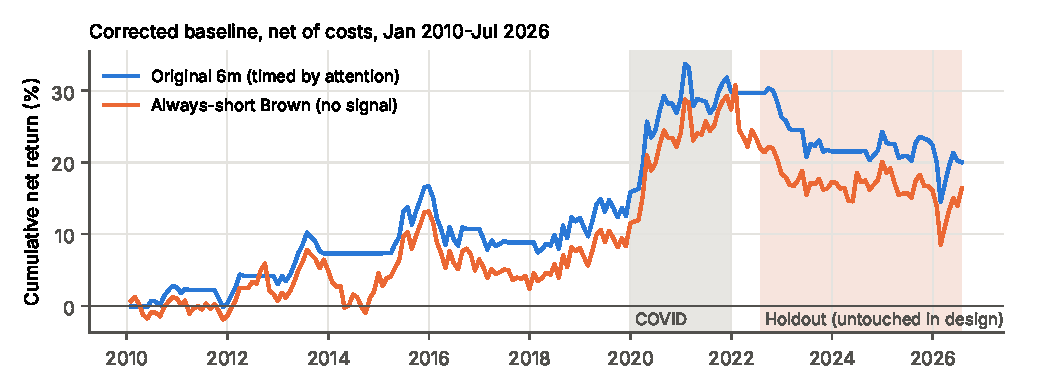
\includegraphics[width=0.86\linewidth]{figures/C1_timed_vs_always_short.pdf}
\caption{Cumulative net return of the 6-month timing rule and the untimed always-short position, January 2010 to July 2026 (corrected baseline). The two lines move together, and both lose in the holdout.}
\label{fig:c1}
\end{figure}

\clearpage
\section{Revision strategy: additional tables}
\label{app:rev}

\begin{table}[!htbp]
\centering\footnotesize
\caption{Monthly Spearman IC (signal at $t$, industry return at $t+1$) with Newey--West (6 lags) $t$. The 1985--2025 column uses only the 492 months where REV exists. Recent 18m = March 2025--August 2026 (REV: 10 months, low power).}
\label{tab:ic}
\fit{tables/T1_ic_summary.tex}
\end{table}

\begin{table}[!htbp]
\centering\footnotesize
\caption{Descriptive IC split (Spearman, NW $t$ in parentheses), REV months only. Chosen after seeing the blend weights. Not part of the test.}
\label{tab:icsub}
\fit{tables/T2_ic_subperiods.tex}
\end{table}

\begin{table}[!htbp]
\centering\footnotesize
\caption{Risk and sizing, mean-variance books, each from its first to its last month. Ex-ante risk is the mean monthly ex-ante active risk. Realized is the annualized volatility of monthly gross returns.}
\label{tab:risk}
\fit{tables/T3_risk.tex}
\end{table}

\begin{table}[!htbp]
\centering\footnotesize
\caption{Mean-variance books, formation months January 1995 to December 2025 (372 months, the only window in which all four books trade). Annualized returns and volatility. Turnover is one-way per month as a fraction of capital. Break-even is the one-way cost at which the mean net return is zero.}
\label{tab:perf}
\fit{tables/T4_performance.tex}
\end{table}

\begin{table}[!htbp]
\centering\footnotesize
\caption{Horizon analysis, net of 20 bp. ``Full'' starts when each book first trades (MOM 1974, blend 1995). Regressions with fewer than 36 months are LOW POWER and not used for the verdict. REV rows are in \texttt{tables/T6\_horizons.csv}.}
\label{tab:hor}
\fit{tables/T6_horizons.tex}
\end{table}

\begin{table}[!htbp]
\centering\footnotesize
\caption{Stress years: compounded net returns (20 bp) of each book and the UMD factor, in \%.}
\label{tab:stress}
\fit{tables/T7_stress.tex}
\end{table}

\begin{table}[!htbp]
\centering\footnotesize
\caption{One-at-a-time robustness grid for the blend, formation months January 1995 to December 2025, net of 20 bp unless the row changes costs. (*) Run on a different cleaned CRSP panel. Not strictly comparable.}
\label{tab:rob}
\fit{tables/T8_robustness.tex}
\end{table}

\begin{table}[!htbp]
\centering\footnotesize
\caption{FF5+UMD alpha (\% a year, NW $t$) by cost level, and the one-way cost at which the gross 6-factor alpha is fully consumed.}
\label{tab:cost}
\fit{tables/T9_alpha_by_cost.tex}
\end{table}

\clearpage
\section{Additional figures}
\label{app:figs}

\begin{figure}[!htbp]
\centering
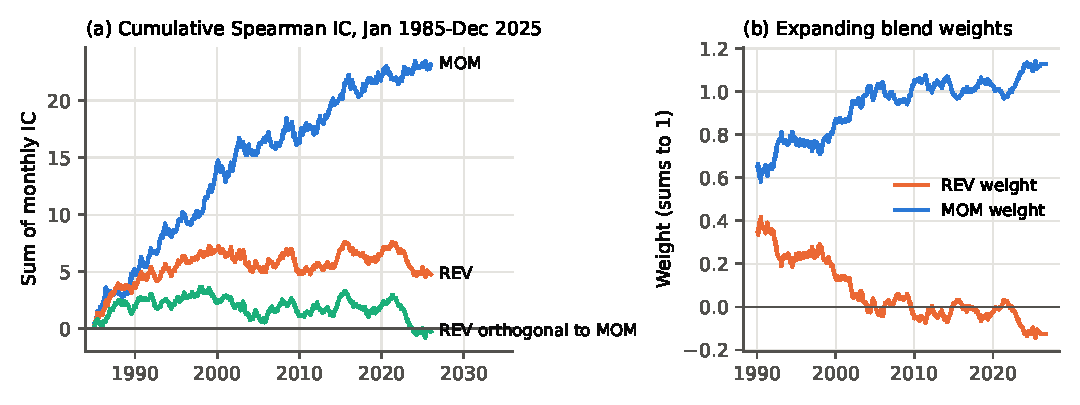
\includegraphics[width=0.9\linewidth]{figures/fig1_ic_and_weights.pdf}
\caption{(a) Cumulative sum of monthly Spearman ICs over the 492 REV months, January 1985 to December 2025. A rising line means positive average IC. (b) Expanding IC-based blend weights, January 1990 to August 2026 (frozen after 2025, when REV is missing).}
\label{fig:ic}
\end{figure}

\begin{figure}[!htbp]
\centering
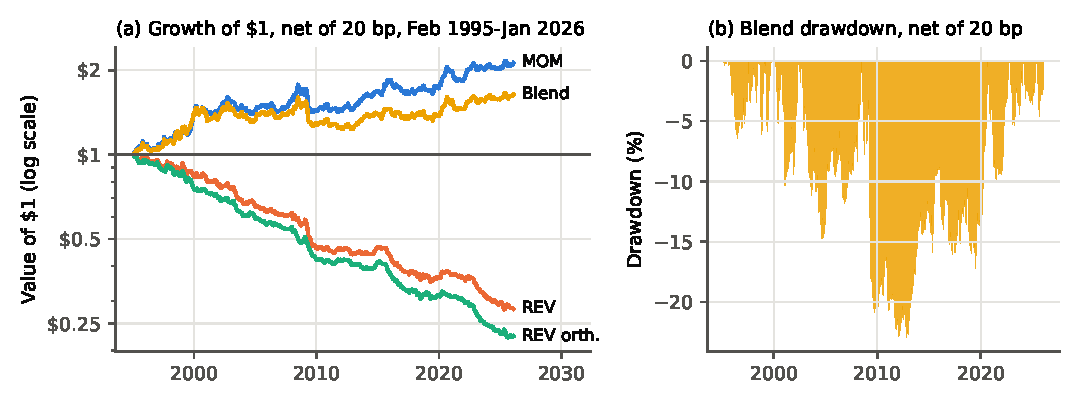
\includegraphics[width=0.85\linewidth]{figures/fig2_cumulative_drawdown.pdf}
\caption{(a) Growth of \$1 in each mean-variance book, net of 20 bp, return months February 1995 to January 2026, log scale. (b) Drawdown of the blended book, net of 20 bp.}
\label{fig:cum}
\end{figure}

\begin{figure}[!htbp]
\centering
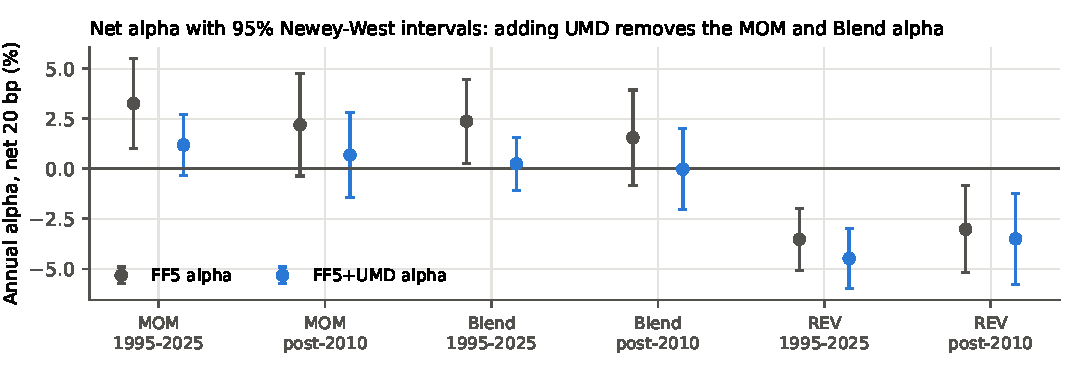
\includegraphics[width=0.85\linewidth]{figures/fig3_alpha_ff5_vs_umd.pdf}
\caption{Annual net alpha (20 bp) with 95\% Newey--West intervals against FF5 (gray) and FF5+UMD (blue), 1995--2025 and post-2010.}
\label{fig:alpha}
\end{figure}

\begin{figure}[H]
\centering
\begin{minipage}[t]{0.58\linewidth}\centering
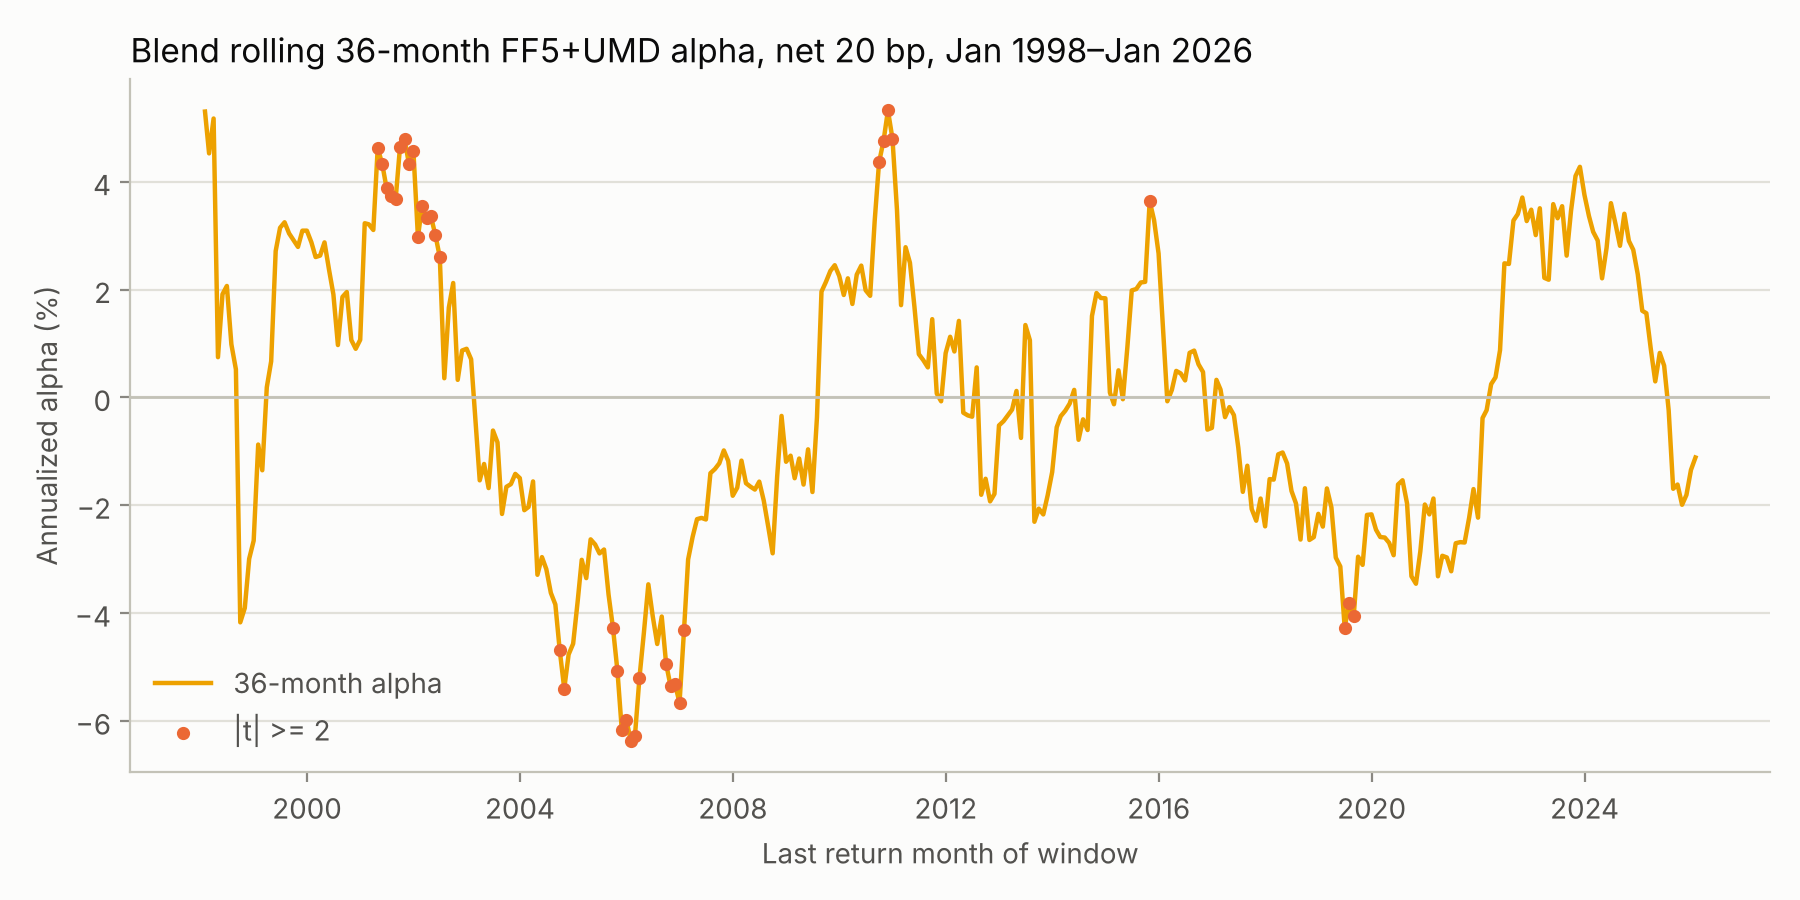
\includegraphics[width=\linewidth]{figures/rolling_alpha_blend.png}
\caption{Rolling 36-month FF5+UMD alpha of the blended book, net of 20 bp, windows ending January 1998 to January 2026.}
\label{fig:roll}
\end{minipage}\hfill
\begin{minipage}[t]{0.38\linewidth}\centering
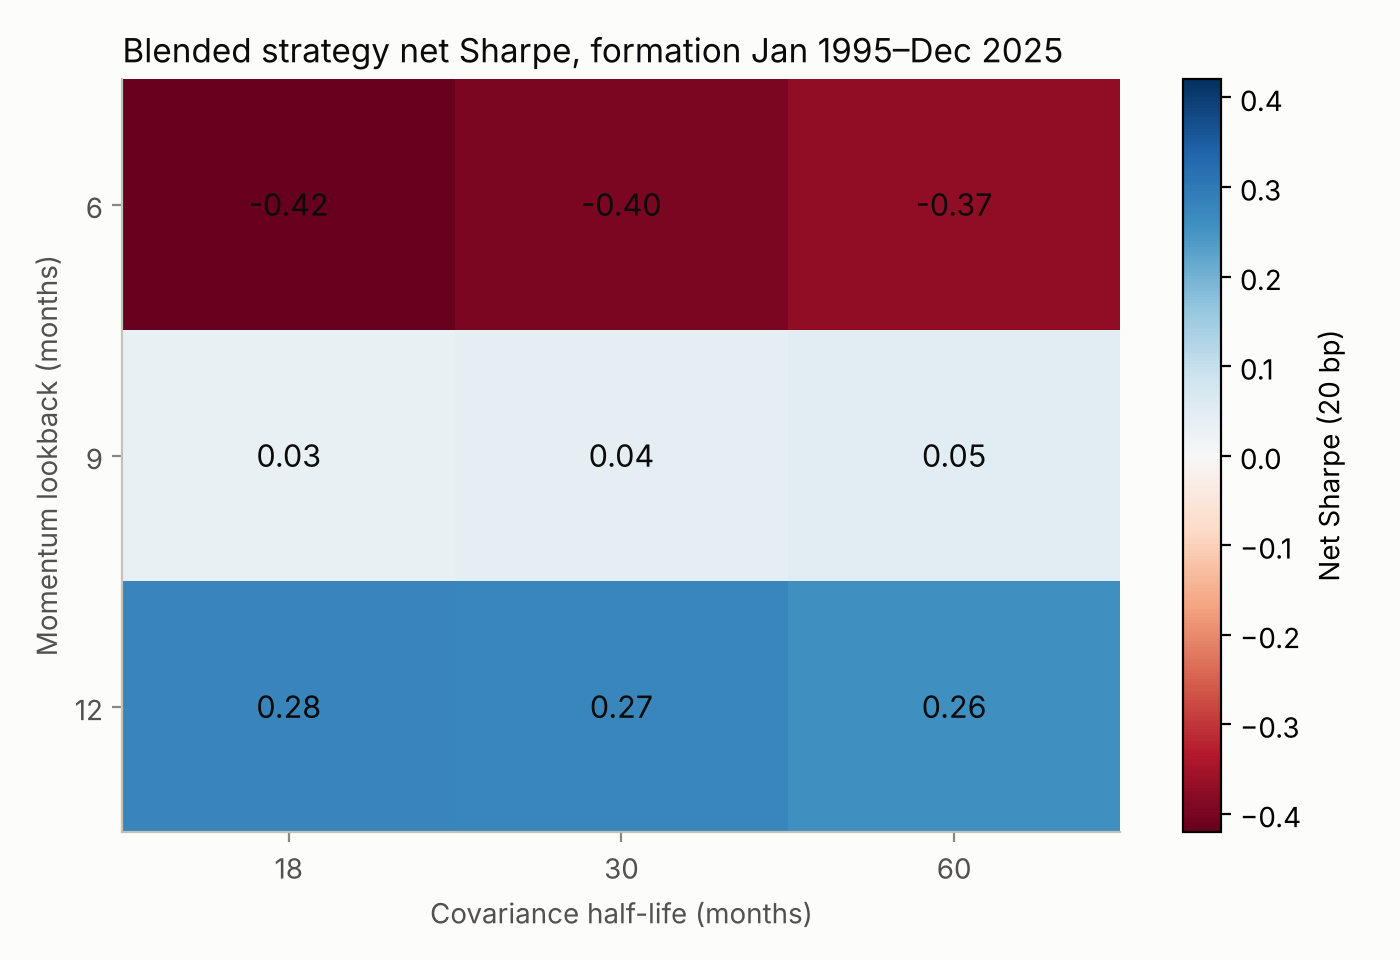
\includegraphics[width=\linewidth]{figures/robustness_heatmap_sharpe.png}
\caption{Net Sharpe (20 bp) of the blended book over momentum lookback and covariance half-life, formation months 1995--2025.}
\label{fig:heat}
\end{minipage}
\end{figure}

\clearpage
\section{Claude interactions, by member}
\label{app:claude}
{\small
% Appendix D: one part per team member. Prompt fragments are generated from
% supporting/transcripts/*/prompt*.md by supporting/code/md_prompts_to_tex.py.

\begin{draftnote}
\textbf{Draft note for the team (delete this box before submission).} This appendix shows the five-conversation structure we agreed on. Two parts are transcripts as sent: D.2 (Hashim's exchange files) and D.5 (the Claude Code log). The prompts in D.1, D.3 and D.4 were re-voiced for this draft from prompts Hashim sent during his audit, so that each facet is asked in its owner's words. The replies they are paired with are the real replies to the original prompts, unchanged, in \path{supporting/transcripts/}. Jack, Cristhian and Aditya: replace these with the prompts you actually sent, or send these and swap in the replies, before anyone signs the report. The dates in those three parts are placeholders.
\end{draftnote}

\subsection*{How to read this appendix}

The brief asks for at least three substantial AI interactions (idea generation, coding support, robustness design), each documented with the prompt, a summary of the output, and a critical evaluation. We have five, one per member, because each of us ran one facet of the project in our own conversation with Claude (Anthropic). D.1 to D.4 were chats with no file access, code execution or web search, so Claude saw only what each prompt contained. D.5 ran in Claude Code against the repository. Every prompt is reproduced verbatim below, the reply is summarized, and the member who sent it evaluates it against what the data later showed. The full replies are in \path{supporting/transcripts/}, one folder per part.

\textbf{Provenance.} No number in this report comes from a Claude reply. Replies proposed tests, code and wording. A member ran the test, compared the code with our own implementation, or checked the wording against the tables before anything was adopted. Where a reply quoted a number it had not computed, we asked it to say so, and it mostly did.

\begin{center}\rule{0.5\linewidth}{0.5pt}\end{center}

\subsection*{D.1 Jack Duncan: design review of the Climate rule (idea generation)}

\textbf{Facet.} I built the attention-timed Short-Brown strategy and the macro-state notebook in the team repository, and asked for a design review before we spent more hours on it. \textbf{Tool and date.} Claude chat, 26 September 2026. Follow-up 28 September. \textbf{Transcript.} \path{supporting/transcripts/D1_jack_design_review/}.

\textbf{Prompt 1 (verbatim).}
\begin{promptbox}
\par\noindent I built the climate-attention timing strategy in our team repo (notebooks/climate\_alpha\_analysis.py) and I want a design review before we sink more hours into it. Act as a skeptical buy-side quant. Find the weak points. Don't fix my prose.
\medskip
\par\textbf{Course context}
\par\noindent MFE 230GA final project, Berkeley. The report needs: a one-paragraph exec summary that says ``Do not implement'' if there is no alpha, ``What did you try'' (idea, data, risk model, turnover/costs, at least three substantial AI interactions), ``What did you learn'' (factor exposures, full sample / post-2010 / last 12-18 months, robustness, critical evaluation of the AI). Grading: thesis 40\%, execution 40\%, originality 20\% (novel data use, prompt design). A clean ``Do not implement'' is fine. Our team of five built the first pass. I own the repo and I'm the one making the changes.
\medskip
\par\textbf{What's in the repo right now}
\par\hangindent=1.2em\hangafter=1\noindent\textbullet~Thesis: Green minus Brown has no permanent premium, but its factor-neutral part pays after spikes in climate-transition attention.
\par\hangindent=1.2em\hangafter=1\noindent\textbullet~Legs: Green = 5 lowest emissions-intensity FF49 industries (Fun, RlEst, Drugs, Telcm, Fin). Brown = 5 highest (Util, Ships, Aero, Steel, BldMt). Equal-weight across value-weighted industries. The emissions file is one static snapshot, 41 of 49 industries (missing Oil, Chips, FabPr, Gold, Hshld, LabEq, Other, Toys).
\par\hangindent=1.2em\hangafter=1\noindent\textbullet~Traded position: short the Brown leg alone (not the spread), with an FF3 overlay from rolling 60-month betas lagged one month.
\par\hangindent=1.2em\hangafter=1\noindent\textbullet~Signal: the attention index (monthly from 1985), as a 60-month rolling z-score of log(1 + attention). Extreme = above the expanding, past-only 80th percentile. Each crossing opens Short-Brown for 3 or 6 months, sized to 5\% residual vol, cap 1x.
\par\hangindent=1.2em\hangafter=1\noindent\textbullet~Costs (assumed): 10 bp on the leg, 5 bp on the market overlay, 25 bp on SMB/HML, per unit of turnover.
\par\hangindent=1.2em\hangafter=1\noindent\textbullet~Variants: ``purified'' attention (the residual from a 120-month walk-forward ridge on rate, oil, inflation and activity shocks). A continuous weight (floor 0.5, 3-month half-life).
\par\hangindent=1.2em\hangafter=1\noindent\textbullet~Validation 2010 to Jul 2022. Holdout Aug 2022 to Jul 2026, frozen.
\medskip
\par\textbf{Numbers (from the notebook)}
\par\hangindent=1.2em\hangafter=1\noindent\textbullet~Validation: the 6-month rules earn about 2.5\%/yr net, FF3 alpha NW t = 2.23 and 2.46. The 3-month rules have t of about 1.5.
\par\hangindent=1.2em\hangafter=1\noindent\textbullet~COVID does the work: the 3-month rule earns 5.94\% net in 2020-21, alpha t = 3.21.
\par\hangindent=1.2em\hangafter=1\noindent\textbullet~Holdout: every version loses 2.1 to 3.8\%/yr (t = -1.7 to -2.2). The IC flips from about -0.08 (negative is the expected sign for a short-Brown rule) to +0.12 to +0.15.
\par\hangindent=1.2em\hangafter=1\noindent\textbullet~2010-2026: the best timed version earns 1.3\%/yr net vs 1.0\% for always-short Brown.
\par\hangindent=1.2em\hangafter=1\noindent\textbullet~The raw spread loads on HML (-0.24 full sample, -0.35 since 2010). After hedging, residual HML is about -0.05 with t of about -2 in every version.
\par\hangindent=1.2em\hangafter=1\noindent\textbullet~Continuous variant: vol down 55-65\%, drawdown down 60-75\%, but the calendar-shuffle placebo gives p of about 0.12.
\par\hangindent=1.2em\hangafter=1\noindent\textbullet~2 of 32 strategy-period cells survive Holm, both in COVID.
\par\hangindent=1.2em\hangafter=1\noindent\textbullet~My macro-state notebook: the attention slope turns positive in high-rate months (difference t = 1.83, Holm p of about 0.6). 47 of those 74 months are in the holdout.
\medskip
\par\textbf{Teammate proposals on the table}
\par\noindent From Cristhian: (A) rebuild with 8 Green and 8 Brown industries. (B) add momentum and an explicit commodity exposure to the controls. (C) regress Fin, Telcm, Drugs, Fun and RlEst one at a time to find where the HML exposure comes from. (D) uniform costs at 5, 10 and 25 bp. From Charishma: (E) a Part B on whether this is alpha or beta at the portfolio level. From the group: (F) macro controls, since exposures look regime dependent (COVID, then inflation and rates). (G) a momentum control, in case the signal is only persistence in past returns.
\medskip
\par\textbf{Data}
\par\noindent In hand: the four team files (FF49 monthly returns, Jul 1926 to Jul 2026, FF3 and rf, the emissions snapshot, a macro file with attention, the 10-year yield, WTI, CPI, CFNAI, the NBER recession flag and GSCPI). Downloadable: Ken French FF5, UMD, short- and long-term reversal, FF49 value- and equal-weighted returns, industry BE/ME, firm counts and average size. FRED Treasury yields (3-month, 2-year, 10-year), BAA and AAA, VIX, commodity indices, activity series, breakevens and TIPS yields. The Gavriilidis Climate Policy Uncertainty index. The Ardia et al. Media Climate Change Concerns index. EPA supply-chain GHG factors by NAICS. No firm-level data. Every result so far starts in 2010, and we have now seen the holdout, so it is spent as a clean test.
\medskip
\par\textbf{What I want back, in this order}
\par\noindent 1. Design critique: max six problems, ranked by how much each could flip the verdict. Problem / why it matters here / fix.
\par\noindent 2. Proposal ranking: one table for A to G: rank, proposal, the result that would change our conclusion, what it can't tell us, overlap with the other proposals, effort in hours. One line of reasoning per row.
\par\noindent 3. New ideas: exactly five, at least two extending the current strategy and at least two alternatives on the same data, each aimed at a small defensible alpha or a more rigorous ``Do not implement''. For each: (a) a falsifiable hypothesis and the result that rejects it. (b) the exact test: sample, return series, specification, benchmark, pass bar. (c) the data, and whether it's in the list above. (d) main pitfalls (look-ahead, multiple testing, small N, overlapping holds). (e) effort in hours. (f) what it adds to the report if it fails.
\par\noindent 4. Plan: the three items from 2 and 3 you'd run first, in order, and why.
\par\noindent 5. The three assumptions in your answer you're least confident about.
\medskip
\par\noindent Rules: work from our numbers, not generic ESG results. Cite a paper only with authors, year and the specific claim. Don't invent backtest results. Label anything you haven't computed as a guess. Under 1,800 words.

\end{promptbox}

\textbf{Prompt 2 (verbatim), sent after we checked reply 1 against the data.}
\begin{promptbox}
\par\noindent Update from our side. We ran most of your proposed tests on the seen data over the weekend. Five of your claims don't hold, and there is a data fact you (and we) missed that changes the review.
\medskip
\par\noindent The attention column is not what we labelled it. Hashim traced it to its source: it is FRED EMVENRGYENVREG, the Baker, Bloom, Davis and Kost Equity Market Volatility tracker for Energy and Environmental Regulation. It counts newspaper articles about stock-market volatility that mention that category, scaled to the VIX. Since 2010 its z-score correlates +0.39 with overall EMV, +0.11 with CPU and -0.06 with MCCC, and 38\% of crossing months are high-EMV months, against 12\% of other months (odds ratio 4.5, p = 0.002). Your coverage worry points the wrong way: the series is exactly zero in 12 of 441 months from 1985-01 to 2021-09, but in 39 of 59 months from 2021-10 (31 of 48 holdout months). The holdout tested a near-binary signal, not the one we validated.
\medskip
\par\noindent Corrections:
\par\noindent 1. Duration. The hedged Brown leg has no holdout rate exposure (d10y t = 0.05), and the strategies gain when yields rise. After FF5 + UMD + d10y + commodity controls, holdout alphas are still -2.3\% to -4.8\% (t about -2).
\par\noindent 2. Newey-West lags. More lags don't shrink the validation t (2.23 at 6 lags, 2.30 at 12). They push the 24-month COVID t to 5.3. The binding problem is small-sample p-values: with t(n-4), 0 of 32 cells survive Holm.
\par\noindent 3. IC flip. It is 1.3 to 1.6 SE for raw and purified, but 2.8 to 2.9 NW SE for the continuous signals.
\par\noindent 4. Idea 1 dates. The frozen rule first crosses in 1993-01 (raw) and 1999-01 (purified).
\medskip
\par\noindent Your tests rescue nothing: timed minus always-on FF5+UMD alpha peaks at t = 1.09, and the Idea 2 post-event CAR is -1.29\% (t = -1.08).
\medskip
\par\noindent Two questions.
\par\noindent (a) Do we salvage this series (as a share of total EMV, or zero-robust) or swap in CPU or MCCC, given both end in 2025 and burn about eight years under our rule? Give me the one rule you'd freeze for the unseen 1993 to 2009 test, its pass bar, and how it treats zeros.
\par\noindent (b) Give me an exact attribution spec that separates timing alpha from duration, value and volatility exposure: dependent variable, regressors, an exposure-matched benchmark, lags, and what counts as alpha.
\medskip
\par\noindent Under 600 words. Flag anything you haven't computed as a guess.

\end{promptbox}

\textbf{Output summary.} Reply 1 (about 1,700 words) opened with a bottom line: the timed rule beats always-on Short-Brown by about 0.3\% a year, so the job is to ``make `Do not implement' airtight, and test pre-specified ideas on the one period nobody has looked at, 1990--2009.'' Its six ranked problems: the benchmark is wrong for a timing claim (``the null is `always short Brown, same hedge, same vol target'''). Validation is one episode, with Aero, Ships and Util taking COVID-specific hits. The holdout is spent, and the IC change is about one standard error. The Brown leg may not measure transition risk (Aero and Ships in the top five is ``surprising'', so rebuild from EPA factors). The holdout loss may be unhedged duration, and inference is weaker than the $t$-statistics suggest (overlapping holds, few events). It ranked the teammate proposals (E first, then A with leave-one-out, G, B, F, C, D), proposed five ideas, three of them extensions (a backward out-of-sample test over 1990--2009, an event-time profile of hedged Brown residuals, the frozen rule on CPU and MCCC) and two alternatives (an all-49 EPA carbon spread, a climate-news hedge portfolio), and named its least-confident assumptions. Reply 2 (about 700 words, over its 600 cap) accepted every correction (``The EMV finding matters more than any of them''), kept ``Do not implement'', and gave one rule to freeze for 1993--2009: the regulation share of overall EMV, zero months treated as missing, the 6-month rule, and a four-part pass bar (timing alpha $t\geq2$ with $t(n-k)$ p-values, calendar-shuffle $p\leq0.05$, at least 8 episodes, the same sign with each Brown industry dropped). It also specified an attribution against an exposure-matched always-short benchmark, with Ferson--Schadt in-position interactions and a 5,000-draw calendar-shuffle null, and declined credit for the holdout: its zero rule ``was written after seeing the holdout, though, so take no credit for that period.''

\textbf{Critical evaluation (Jack).} The first reply was a competent design review of a variable it never looked at. We scored 52 checkable claims: 26 right, 15 partly right, 6 wrong, 5 unverifiable. Three things changed our plan. First, critique 1: I had tested timed returns against zero, when the null for a timing claim is the always-short position with the same hedge. On the seen data that settles it (timed minus always-short FF5+UMD alpha peaks at $t=1.09$). Second, the backward test on the pre-2010 window was not in my plan and became the frozen test in D.2. Third, it flagged Aero and Ships as odd Brown members and guessed that Aero, Util and Ships drove the COVID gains. Both held (EPA factors rank them 31st and 20th of 49, and those three industries deliver 86\% of the 3-month rule's COVID gross P\&L). Six claims were wrong. The holdout was not lost to duration: the hedged leg has no holdout rate exposure ($\Delta$10y $t=0.05$), and alphas stay at $-2.3\%$ to $-4.8\%$ after rate and commodity controls. More Newey--West lags do not fix inference. They push the 24-month COVID $t$ to 5.3, and the binding problem is small-sample p-values. The IC flip is 1.3 to 1.6 standard errors for the raw signal, not ``about one''. Its dates for the backward test were wrong, and it put the coverage risk in the wrong period. The bigger miss is one we share: neither reply asked what ``attention'' measures, and neither did my prompt. I passed on the label from our macro file without a source. Hashim traced it to FRED the same week, and our follow-up relayed his finding. The follow-up turned corrections into specifications: the frozen rule and the exposure-matched attribution went into the project almost as written, with three fixes (the two zero thresholds were redundant, the share signal keeps most of the original timing, and $k=14$ undercounted 15 coefficients). \textbf{Where it went:} the always-short benchmark (Section~2.1), the frozen 1994--2009 test (D.2), the EPA rebuild and the MCCC/CPU placebos (Appendix~A).

\begin{center}\rule{0.5\linewidth}{0.5pt}\end{center}

\subsection*{D.2 Hashim Almodamagha: code for the frozen 1994--2009 test (coding support)}

\textbf{Facet.} I traced the attention column to FRED EMVENRGYENVREG, wrote the pre-registration for the one window nobody had backtested, and asked Claude for an independent implementation of the frozen rule to run against mine. \textbf{Tool and date.} Claude chat, 26 September 2026 (both messages). \textbf{Transcript.} \path{supporting/transcripts/D2_hashim_frozen_test_code/}.

\textbf{Prompt 1 (verbatim).}
\begin{promptbox}
\par\noindent Write Python code for a pre-registered backtest I will run exactly once. You do not have the data, so report no results.
\medskip
\par\noindent CONTEXT. This is my MFE 230GA final project at Berkeley. Our team's strategy shorts a factor-hedged ``Brown'' industry leg after attention spikes. It failed its 2022-2026 holdout, and we recommend ``Do not implement''. I froze one rule for 1993-2009, the one tradable window nobody has backtested. I will debug your code on synthetic data and the seen 2010-2022 window first, so the test window is a parameter and nothing is tuned.
\medskip
\par\noindent INPUTS. Returns are monthly decimals.
\par\noindent 1. \texttt{ff49\_industry\_monthly.csv}: a \texttt{date} column (month-end, e.g. 1926-07-31) and 49 Fama-French industry columns of value-weighted returns, NaN before an industry exists. Brown = Util, Ships, Aero, Steel, BldMt. The Brown leg R\^{}B\_t is their equal-weighted mean minus RF.
\par\noindent 2. \texttt{fac}: a DataFrame parsed from Ken French's FF5 and momentum files, month-end DatetimeIndex from 1963-07, columns Mkt-RF, SMB, HML, RMW, CMA, RF, UMD.
\par\noindent 3. FRED CSVs with columns \texttt{observation\_date} (first of month; map to month-end) and the series id: EMVENRGYENVREG and EMVOVERALLEMV (monthly from 1985-01; the first has exact zeros, the second none), GS10 (monthly average 10-year yield, percent), MCOILWTICO (monthly average WTI price, from 1986-01), VIXCLS (daily closes from 1990-01-02, blank on holidays).
\medskip
\par\noindent THE TEAM TRADE (validated, unchanged).
\par\hangindent=1.2em\hangafter=1\noindent\textbullet~Hedge: OLS of R\^{}B on a constant and f = (Mkt-RF, SMB, HML) over months t-59 to t gives (a\_t, b\_t); residual e\_t = R\^{}B\_t - a\_\{t-1\} - b\_\{t-1\}'f\_t.
\par\hangindent=1.2em\hangafter=1\noindent\textbullet~Size: m\_t = min(1, 0.05 / (sqrt(12) * sd\_t)), sd\_t = 36-month rolling std (ddof=1) of e through t.
\par\hangindent=1.2em\hangafter=1\noindent\textbullet~Position w\_t = -m\_t in a hold month, else 0, set at the end of month t; it earns w\_t*R\^{}B\_\{t+1\} - w\_t*b\_t'f\_\{t+1\}.
\par\hangindent=1.2em\hangafter=1\noindent\textbullet~Costs per unit of turnover: 10 bp on |$\Delta$w|, 5 bp on the Mkt-RF overlay change, 25 bp on SMB and HML overlay changes; a trade at the end of t pays in t+1.
\par\hangindent=1.2em\hangafter=1\noindent\textbullet~A crossing is an extreme month whose previous month was not extreme. The hold covers the crossing month and the next five. With the publication lag, the hold state at the end of t uses the extreme flag of t-1.
\par\hangindent=1.2em\hangafter=1\noindent\textbullet~Always-on benchmark R\^{}AO: every month is a hold month.
\medskip
\par\noindent THE FROZEN RULE.
\par\noindent 1. Signal: s\_t = EMVENRGYENVREG\_t / EMVOVERALLEMV\_t, observed one month late (the value for month t is usable at the end of month t+1).
\par\noindent 2. Zeros: a zero month is missing, not low attention. It cannot trigger a position, and it is dropped from both the z-score window and the percentile history. The z-score needs at least 48 nonzero months in the trailing 60; if more than 10\% of the trailing 60 months are zero, the signal is off.
\par\noindent 3. Extreme month: z\_t = 60-month rolling z-score of log(s\_t) over nonzero months; extreme when z\_t exceeds its expanding, past-only 80th percentile (team convention: at least 60 prior z observations).
\par\noindent 4. Trade: the 6-month rule above. A new crossing during a hold extends the hold; positions never stack.
\par\noindent 5. Sample: 1993-01 to 2009-12 (or from the first month the rule can fire, if later), run once.
\par\noindent 6. Pass bar, all four required: (i) the timing alpha below is positive with t \textgreater{}= 2 and p from t(n-k); (ii) calendar-shuffle p \textless{}= 0.05 (move the same hold windows to random dates, 5,000 times, recompute alpha); (iii) at least 8 independent episodes (merge holds that touch or overlap); (iv) alpha keeps its sign when each Brown industry is dropped in turn (rebuild leg, hedge, sizing, R\^{}AO and pi each time).
\medskip
\par\noindent ATTRIBUTION. D\_t = R\^{}T\_t - pi*R\^{}AO\_t, net of costs, with R\^{}T the timed strategy and pi = mean |timed position| / mean |always-on position| over the test window. Regress D\_t on FF5 + UMD, BOND, the WTI log return, dVIX\_t (change in the monthly mean of daily VIX), dlog EMVOVERALLEMV\_t, and I\_\{t-1\} x \{Mkt-RF, HML, BOND, dVIX\}, where I\_\{t-1\} = 1 if the strategy held a position entering month t. Alpha is the intercept. Newey-West with 6 lags (12 as a check); p from t(n-k), k = number of estimated parameters. Report mean(D) = alpha + sum beta*mean(F) + sum gamma*mean(I*F).
\medskip
\par\noindent BOND is the monthly excess return of a constant-maturity 10-year Treasury from GS10 (percent to decimal): r\_t = y\_\{t-1\}/12 - D\_\{t-1\}*(y\_t - y\_\{t-1\}) + 0.5*C\_\{t-1\}*(y\_t - y\_\{t-1\})\^{}2, with D and C the modified duration and convexity of a 10-year semiannual par bond at yield y\_\{t-1\}, minus RF.
\medskip
\par\noindent CONSTRAINTS.
\par\hangindent=1.2em\hangafter=1\noindent\textbullet~No look-ahead: every input used at the end of month t is known then (the signal a month later). Attribution regressors are contemporaneous by design; do not lag them.
\par\hangindent=1.2em\hangafter=1\noindent\textbullet~pandas, numpy and statsmodels only. \texttt{sm.OLS(...).fit(cov\_type=``HAC'', cov\_kwds=\{``maxlags'': 6\}, use\_t=True)} matches our team's Newey-West t and gives p from t(n-k). Count k from the design matrix.
\par\hangindent=1.2em\hangafter=1\noindent\textbullet~One function per step, each with a docstring giving inputs, outputs and timing convention. Fixed seed, no parameter search, no plots.
\medskip
\par\noindent Where the spec is silent, pick one reading, make it a parameter and say why. Three I see: whether a zero month between two extreme months makes the next one a new crossing; how the shuffle places windows and whether pi and I are recomputed per draw; what happens to a hold still open in 2009-12.
\medskip
\par\noindent OUTPUTS, as DataFrames, also printed.
\par\noindent 1. Pass/fail table: one row per component (i) to (iv), with statistic, bar, value, pass/fail; then the overall verdict.
\par\noindent 2. Attribution: coefficient, NW(6) t, NW(12) t and p per regressor; n, k, R-squared, pi, window dates.
\par\noindent 3. Decomposition: mean(D), alpha, every beta*mean(F) and gamma*mean(I*F) term, and the identity gap (zero to machine precision).
\par\noindent 4. Diagnostics: first month the rule can fire, zero-month counts, crossing dates, episode list, leave-one-out alphas and t.
\par\noindent 5. Shuffle: actual alpha, null quantiles, p.
\medskip
\par\noindent AFTER THE CODE.
\par\noindent (a) Number every assumption you made beyond this spec.
\par\noindent (b) The checks you would run before my single real run, each with the result that would make you stop, including a look-ahead test.

\end{promptbox}

\textbf{Prompt 2 (verbatim), sent after running reply 1 on the real data.}
\begin{promptbox}
\par\noindent I ran your script on the real data and through your checks. It ran the first time, with only file paths and \texttt{fac} supplied, and reaches the same verdict as my own implementation (FAIL, 1 of 4). The numbers differ, and one of your stop rules fires.
\medskip
\par\noindent 1. \texttt{make\_synthetic\_inputs}. GS10 is a random walk clipped at 0.5 that sits on the floor (76\% of 1995-2009 months for seed 0, every month for seed 16). BOND is then constant, I x BOND acts as an I main effect, and your positive control fails check (b)10: 4\% of the planted 3\% effect reaches alpha (t 0.98), while I x BOND has t -10.8. Seed 16 crashes the null-seed loop (rank-deficient design).
\medskip
\par\noindent 2. \texttt{attention\_signal}. Requiring 60 full calendar months before the first z is a silent reading you hard-coded. I treat pre-1985 months as unavailable, not zero, so the 48-nonzero minimum is the burn-in. Your reading moves the first threshold from 1994-01 to 1994-12, adds a 2002-12 crossing and starts the window at 1995-02, not 1994-03: pi 0.809 vs. 0.729, shuffle p 0.536 vs. 0.478.
\medskip
\par\noindent 3. \texttt{leg\_pipeline}. You hedge with the Mkt-RF, SMB and HML in \texttt{fac}, the FF5 file. The team hedge uses its FF3 file, which my prompt never said (my gap). SMB differs by up to 3.5 pp a month, b\_t moves by up to 0.09, and your check (b)2 stops at 2.3e-3 a month (6e-17 with FF3).
\medskip
\par\noindent 4. \texttt{pass\_fail\_table}. (iv) passes a negative alpha whose five drop-one alphas are also negative.
\medskip
\par\noindent With readings 2 and 3 switched to mine, your code matches my implementation to 1e-13, all 5,000 shuffle draws included.
\medskip
\par\noindent Two smaller gaps. \texttt{check\_no\_lookahead} compares end-of-T states only, so it missed both return-side bugs I injected (month-t return hedged with b\_t; a position earning its own month). Seen mode ends at 2022-12; its five holdout months flip the seen alpha from -0.16\%/yr (t -0.24) to +0.26\%/yr (t 0.37).
\medskip
\par\noindent Please send corrected versions of these functions only, each with a unit test:
\par\hangindent=1.2em\hangafter=1\noindent\textbullet~\texttt{make\_synthetic\_inputs}: BOND varies in every window for seeds 0-20, and the positive control puts at least 80\% of the planted shift in alpha with t \textgreater{} 2.
\par\hangindent=1.2em\hangafter=1\noindent\textbullet~\texttt{attention\_signal}: a \texttt{z\_burn\_in} parameter with both readings; on a zero-free series from 1985-01, the first z falls in month 48 under mine and month 60 under yours.
\par\hangindent=1.2em\hangafter=1\noindent\textbullet~\texttt{leg\_pipeline}: a separate \texttt{hedge\_fac} input; changing its SMB moves b\_t but not the attribution regressors.
\par\hangindent=1.2em\hangafter=1\noindent\textbullet~\texttt{pass\_fail\_table}: a negative alpha fails (iv).
\par\hangindent=1.2em\hangafter=1\noindent\textbullet~\texttt{check\_no\_lookahead}: a return-side comparison that flags both injected bugs.
\par\hangindent=1.2em\hangafter=1\noindent\textbullet~\texttt{\_\_main\_\_}: seen mode ends at 2022-07, with \texttt{cut\_to} on its look-ahead call.
\medskip
\par\noindent These fixes are for reproducibility; the frozen rule stays.

\end{promptbox}

\textbf{Output summary.} Reply 1 returned one self-contained 985-line script (pandas, numpy, statsmodels), stating up front: ``I have not executed this code. Treat the checks in (b) as mandatory before the single real run.'' A frozen \texttt{Config} holds every number. Each step is one function with a docstring that states its timing (lagged hedge, publication lag, holds that extend but never stack, costs paid in $t+1$). The three silent points I named became parameters with reasons (bridge a zero month between two extreme months, for at most six months, recompute $\pi$ and the in-position indicator in every shuffle draw, truncate a hold still open at the window end). It numbered 25 assumptions beyond the spec, four of which mattered later (a 60-calendar-month burn-in, a window starting ``roughly 1995-02 rather than 1993-01'', no in-position main effect, ``keeps its sign'' read as the same sign as the full-sample alpha), and listed 13 pre-run checks with stop rules, including a truncation look-ahead test, a planted-effect positive control, 20 null seeds and a SHA-256 freeze. Reply 2 returned six corrected functions with one unit test each (a stationary synthetic yield so the positive control works, a \texttt{z\_burn\_in} parameter with both readings, a separate \texttt{hedge\_fac} input that refuses the FF5 file, criterion (iv) requiring all drop-one alphas positive, a look-ahead audit that perturbs inputs at month $T$ and checks positions and returns, seen mode ending 2022-07), and said again: ``Please run the tests before anything else.''

\textbf{Critical evaluation (Hashim).} The first reply wrote a correct backtest inside a flawed test harness. I never used it as the run of record: I ran it on the real data as a second implementation and compared every component with my own, which reproduces the team pipeline bitwise. The core mathematics matched. The script ran the first time, with only file paths supplied, and reached my verdict (FAIL, 1 of 4, with alpha $-0.19\%$ a year, $t=-0.25$, against $-0.18\%$, $t=-0.27$). Two readings explain every numeric gap. With both switched to mine it reproduces all 15 coefficients, the drop-one alphas and all 5,000 shuffle draws to $3.3\times10^{-13}$. Three of the six problems came from my prompt: it described only the FF5 factor frame, so the code hedged with FF5 SMB (up to 3.5 pp a month off the team FF3 SMB), ``keeps its sign'' let criterion (iv) pass a negative alpha, and ``the seen 2010--2022 window'' let seen mode run to 2022-12, where five holdout months flip the seen alpha from $-0.16\%$ ($t=-0.24$) to $+0.26\%$ ($t=0.37$). The other three were its own: a hard-coded burn-in that it disclosed but should have parameterized (window start 1995-02 instead of 1994-03, shuffle $p$ 0.536 instead of 0.478). A synthetic 10-year yield that sat on its floor, so the positive control failed its own stop rule (4\% of the planted effect reached alpha), and a look-ahead test that compared end-of-month states only and missed the two return-side bugs among six I injected. The follow-up fixed all six (every unit test passed first time, the positive control now puts 97--104\% of the planted shift in alpha, the new audit flags 7 of 8 injected bugs) and broke one interface, because I sent it in a fresh chat without the first reply, so it rewrote functions it could not see. A literal drop-in crashes. The repaired harness also audited our own inference: on 100 null seeds the calendar shuffle is correctly sized (6 rejections at 5\%), but the NW(6) $t$ over-rejects (13), a bias that cannot rescue a negative alpha. Trust its formulas and audit its interfaces: run against a reference and never trusted blind, Claude is a cheap second implementation of backtest code, not a verifier of it. \textbf{Where it went:} the frozen test's second implementation (Appendix~A, row 4), the size check that qualifies every NW(6) $t$ in Section~2.3.

\begin{center}\rule{0.5\linewidth}{0.5pt}\end{center}

\subsection*{D.3 Cristhian Ruiz Cardozo: the multiple-testing framework (robustness design)}

\textbf{Facet.} I ran the four tests I had proposed at the halfway point (8-and-8 legs, FF5+UMD+commodity controls, the source of the HML loading, uniform costs), which produced a grid of 8,091 alpha tests, and then asked Claude how a project with 23,923 logged tests should decide its verdict. \textbf{Tool and date.} Claude chat, 30 September 2026. \textbf{Transcript.} \path{supporting/transcripts/D3_cristhian_multiple_testing/}.

\textbf{Prompt (verbatim).}
\begin{promptbox}
\par\noindent Please act as the skeptical member of an investment committee. The task is to design the robustness and multiple-testing framework that will decide the final verdict of our project. All the information you need is given below. Please do not ask for data.
\medskip
\par\noindent Setting. This is the MFE 230GA (Active Asset Management, UC Berkeley) final project. The grading weights are 40\% thesis, 40\% execution and 20\% originality, and the brief requires ``Do not implement'' when there is no alpha. Our team's thesis: short a Brown industry leg (Util, Ships, Aero, Steel, BldMt, from the Fama-French 49), hedged with rolling 60-month FF3 betas, for 3 or 6 months after ``climate-transition attention'' crosses its expanding 80th percentile. There are six variants: a raw or macro-purified signal with either hold, or a continuous weight. Validation is 2010-01 to 2022-07. The holdout is 2022-08 to 2026-07. Our provisional verdict is Do not implement. The team ran eight analysis modules, and an independent re-implementation reproduced each one. Each module names its primary tests in its code. Only the 1994-2009 rule (item 7) has a hash and timestamps proving that its tests were fixed first.
\medskip
\par\noindent Evidence (annualized, Newey-West(6) t, p from t(n-k)).
\par\noindent 1. Team record. Validation: the 6-month rules earn FF3 alphas of 2.1\% to 2.5\% (t 2.2 to 2.6). Holdout: all six lose 0.5\% to 3.8\% a year net (FF3 alpha t down to -2.19), and the IC flips from -0.09 to +0.12. Audit: the team's ``2 of 32 cells survive Holm'' were two 24-month COVID regressions with normal p-values (0 of 32 with t(n-4)). A missing October 2025 CPI print created the whole Pure-versus-Original holdout gap. The emissions file has no source, units or date.
\par\noindent 2. The signal is FRED EMVENRGYENVREG, a volatility-news tracker for energy and environmental regulation. Its z-score correlates -0.0004 with the Ardia et al. Media Climate Change Concerns index (MCCC) and 0.12 with climate policy uncertainty (CPU), through overall volatility news (partial r 0.05). It is exactly zero in 31 of 48 holdout months.
\par\noindent 3. MCCC and CPU in the identical machinery: 0 of 12 validation alphas reach t 1.96 (EMV: 4 of 6), all six MCCC holdout alphas are negative, and the smallest Holm p over 40 primary tests is 1.00. A signal-free always-short Brown position earns 71\% of the COVID alpha.
\par\noindent 4. My own four tests (8-and-8 legs, FF5+UMD+commodity controls, the source of the HML loading, uniform 5/10/25 bp costs): 8,091 alpha tests, 0 positive survivors under Holm or BH. 0 of 900 attention-rule holdout alphas are positive.
\par\noindent 5. Alpha versus beta. A traded 10-year Treasury factor (BOND) plus UMD makes every holdout alpha slightly more negative. Rates moved holdout returns by 0.5 pp a year at most. The Lewellen-Nagel beta-timing term is negative (-0.6\% to -1.1\%), and the always-short benchmark carries it too. The COVID gain is market and size exposure that the lagged hedge left open.
\par\noindent 6. Emissions. On EPA supply-chain intensities Aero and Ships rank 31st and 20th of 49 (in the team file: 3rd and 2nd of 41). The EPA-ranked Green-minus-Brown spread earns 6.4\% post-2010 (t 1.72) and 9.6\% in the holdout (t 1.61), but its pre-specified FF5+UMD alpha is 4.7\% (t 1.52). Its full-sample alpha, 4.5\% (t 2.58), comes from short CMA and UMD loadings and from a 2022 sort applied back to 1970.
\par\noindent 7. Frozen rule. A pre-registered EMV-share rule, scored once on the unseen 1994-03 to 2009-12 window, fails 3 of 4 pass-bar components: alpha -0.18\% (t -0.27), calendar-shuffle p 0.48.
\par\noindent 8. Shrinkage timing (a Lehnherr-Mehta-Nagel style ridge). Cross-validation picks the maximum penalty in 100\% of monthly refits, so every forecast is the historical mean. Attention lowers out-of-sample $R^2$ at every fixed penalty.
\par\noindent 9. Carbon-aware industry momentum (8 long, 8 short, t-12 to t-2, 10 bp). Net Sharpe 0.47, but the pre-registered FF5+UMD alphas are 1.74\% (t 1.09) and 1.86\% post-2010 (t 0.71), with UMD beta 0.99. A Grinold-Kahn optimizer book (IC fixed at 0.05, 5\% ex-ante tracking, and its alpha was exploratory) has a full-sample alpha of 2.17\% (t 3.07, BH p 0.027) and an IR of 0.555, a post-2010 alpha of 3.12\% (t 2.18), but a holdout alpha of -0.34\% (t -0.15). Rank IC: 0.054 full sample, 0.030 holdout. Carbon frontier: at bound b = -1 the long leg's carbon intensity falls 60\% for an IR change of -0.005 (95\% CI -0.110 to +0.096). Only b = -2 costs significantly (-0.284, p 0.038).
\medskip
\par\noindent Test count. The eight ledgers hold 23,923 tests: 155 primary, 8,113 robustness, 15,485 exploratory, 170 placebo or reference. About 4,200 have nominal p \textless{} 0.05, many of them factor loadings. They overlap heavily: shared holdout months, near-identical variants, and one grid of 8,091 alphas.
\medskip
\par\noindent Unseen data. FF49 returns start in 1926-07 and FF5 in 1963-07, but no module computed a strategy return before 1970.
\medskip
\par\noindent Questions, to be answered under these headings.
\par\noindent Question 1, families. How should the family-wise error rate or the false discovery rate be controlled across a project of this size? Which families should be defined, which should receive Holm or Romano-Wolf and which BH or BY, whether loadings and descriptive tests belong in any family, and how dependence between near-duplicate variants should be treated.
\par\noindent Question 2, deflated Sharpe. How should the best Sharpe ratios be deflated for the number of trials? Which ratios, what counts as a trial, how the effective number of independent trials should be estimated, and every input the formula needs. Available: the optimizer book (679 months, annualized Sharpe 0.555, skew -0.28, raw kurtosis 5.77, and post-2010: 199 months, 0.70, 0.29, 3.66) and the EPA spread (post-2010: 0.52, 0.35, 4.77).
\par\noindent Question 3, candidates. At most two that deserve the strictest scrutiny, and the exact tests that would move each one to ``implement'': sample, benchmark, statistic, pass bar.
\par\noindent Question 4. The one robustness check most likely to overturn ``Do not implement'', and the result that would do it.
\par\noindent Question 5. What an investment committee would still object to after all of this.
\par\noindent Question 6. A prioritized checklist of at most ten items: test, pass bar, and what a fail means.
\medskip
\par\noindent Conditions. Please work from these numbers only. Cite a paper only with authors, year and the specific claim. Label any number you have not computed as a guess. Do not propose new signals. ``No candidate can reach implement'' is an acceptable answer, provided you say why. Please keep the answer under 1,500 words.

\end{promptbox}

\textbf{Output summary.} The reply (about 1,700 words, over its 1,500 cap) opened with its bottom line: ``no candidate reaches `implement' on the current evidence. The attention thesis is finished.'' Families: ``Group tests by the decision they could change, not by module''. A one-sided confirmatory family holding only each candidate's pre-specified alpha test, controlled by Romano--Wolf on a stationary block bootstrap with Holm alongside. My 8,091 alphas as a sensitivity analysis under BH or BY, reported as a distribution. No family for loadings, descriptive statistics or placebos. For near-duplicate variants a max-$t$ bootstrap or Nyholt's $M_{\mathrm{eff}}$, and for best-of-many claims White's Reality Check or Hansen's SPA. Deflated Sharpe: the PSR and DSR formulas of Bailey and L\'opez de Prado (2014) with every input, applied to the optimizer book's Sharpe, its appraisal ratio (``with a UMD beta of 0.99 the raw Sharpe is mostly momentum'') and the EPA spread, with a hand-computed table (book DSR 0.99, 0.94, 0.81 at $N=10$, 100, 1,000, and EPA spread 0.71 at $N=10$, failing even at $N=2$). Candidates: the carbon-aware optimizer book, with a frozen, hashed run on 1927--1969 against FF3+UMD and a four-part pass bar, and the EPA spread, whose ``only route is live paper-trading''. The one check that could overturn the verdict: the frozen pre-1970 run, and even a pass ``would justify only `implement at pilot size with paper-trading'''. Committee objections: ``it is just momentum'', crash risk, low power, unverifiable pre-registration, data provenance, untested costs above 10 bp, one regime in the holdout. A ten-item checklist closed it.

\textbf{Critical evaluation (Cristhian).} The reply's statistics hold up. Its reading of our books does not. We scored 93 claims: 67 correct, 15 partly correct, 11 wrong. Every formula and citation checks out, all ten cells of its deflated Sharpe table reproduce to within 0.005, and its bottom line matches ours. The framework is what we kept: families defined by the decision a test could change, so that loadings, placebos and exploratory rows sit outside every family. The appraisal ratio, not the raw Sharpe, as the ratio to deflate (the optimizer book earns 4.53\% over FF5 but 2.17\% once UMD enters). A max-$t$ or SPA test for any best-of-many claim, and a single frozen run on the book's one untouched window, 1931--1969. Of the eleven wrong claims, three trace to my prompt: I printed the equal-weight book's UMD beta (0.99) beside the optimizer's numbers, and two of its claims rest on it (the optimizer loads 0.27, $t=15.2$). I never named the book's carbon source, so it guessed ``2022 intensities''. The other eight are its own. Romano--Wolf is not stricter than BH on our grid. Loadings are 32\% of the nominal hits, not ``most''. We had tested 25 bp. Its window cannot start before 1931-07, since the optimizer needs 60 months. And ``insufficient evidence, not evidence of no alpha'' is false for the attention thesis: each of the six rules rejects a $+2\%$ holdout alpha at one-sided $p\leq0.0016$. Several of its pass bars would have misread our data. The DSR clause in its pre-1970 bar is decided by post-1970 data and fails on its own arithmetic beyond 7 trials. Its $\pm2\%$ equivalence test calls a significantly negative holdout ``insufficient evidence''. Its MCCC control raises the EPA spread's alpha, and ``no significant carbon cost'' rewards low power. It also missed the conflict between its own yardsticks: at 42 effective trials a 5\% max-$t$ bar is 3.03 and a 0.95 DSR needs about 3.85, and the book's $t$ of 3.07 sits between them with no rule for which governs. We adopted the sorted families, one-sided Holm and BH on the 73 distinct primary alphas, BH and BY on the grids, the deflated appraisal ratio required in both windows, and the frozen run with three pre-set readings, with one rule it lacked: max-$t$ decides whether an alpha survives the search, and only the DSR can move a verdict. The frozen run passed (1.95\% a year over FF3+UMD before 1970, $t=2.45$), but the deflated appraisal ratio is 0.559 and the holdout alpha $-0.34\%$, so the book moves to paper trading at pilot size and the verdict holds. \textbf{Where it went:} Section~2.3 (multiple testing), Appendix~A rows 5 and 6.

\begin{center}\rule{0.5\linewidth}{0.5pt}\end{center}

\subsection*{D.4 Aditya Aryan: red team of the Climate verdict (critical review, two rounds)}

\textbf{Facet.} My job was to attack our own conclusion before a grader did. I sent Hashim's draft summary of the Climate verdict with the claims behind it, checked the reply against our files, and sent the rewritten summary back with the best evidence against us. \textbf{Tool and date.} Claude chat, 1 and 2 October 2026. \textbf{Transcript.} \path{supporting/transcripts/D4_aditya_red_team/}.

\textbf{Prompt, round 1 (verbatim).}
\begin{promptbox}
\par\noindent I'm the red team on my own team's report. Read Hashim's draft verdict twice: once as the investment-committee member who has to sign ``Do not implement'', once as a journal referee. Break it before the grader does. No summary. No praise. If a sentence is weaker than its evidence, say so.
\medskip
\par\noindent Context: UC Berkeley MFE 230GA final project (thesis 40\%, execution 40\%, originality 20\%). The ``What did you learn'' section is at its page limit, so any edit there has to replace text, not add it.
\medskip
\par\noindent Here is the draft executive summary of the Climate section, as Hashim wrote it:
\medskip
\par\noindent ``Our team's halfway project proposed a state-dependent climate trade: short the factor-hedged Brown industry leg (Util, Ships, Aero, Steel, BldMt) for three or six months after ''climate-transition attention`` crosses its past-only 80th percentile, sized to 5\% residual volatility. Its best-specified form, which I froze before testing it, triggers on the energy-and-environmental-regulation share of volatility news, lagged one month. I asked three questions of the strategy: what the signal measures, what the legs are, and whether any version survives a window it was not designed on. The study uses Fama-French industry and factor returns, FRED news and macro series, two climate-concern indices (MCCC and CPU) and EPA supply-chain emission factors; every inference uses real-time inputs and small-sample p-values, each module fixes a primary test, and an independent verifier rebuilt each module's headline numbers. The recommendation is Do not implement, for four reasons. First, the ''attention`` series is FRED's equity-volatility news tracker for energy and environmental regulation (identical in 500 of 500 months), its z-score is uncorrelated with media climate concern (r = -0.0004), and the same machinery fed genuine climate measures earns 0 of 12 validation alphas with t \textgreater{}= 1.96. Second, the rule frozen before its test window earns -0.18\% a year over 1994-2009 (t = -0.27, shuffle p = 0.48). Third, the COVID gain belongs to the position: an untimed short of the same leg earns 71\% of it, and the rule's edge over that short is +1.84\% a year (t = 0.87). Fourth, every timed rule has a negative 2022-2026 holdout alpha in all 900 net-of-cost configurations, all 28 zero-cost runs are negative too, and rates do not explain the loss. Carbon-aware industry momentum and shrinkage-based timing on the same data fare no better. In short: read the label, benchmark timing against the always-on position, and spend the last clean window on one frozen rule.''
\medskip
\par\noindent The claims behind it (Newey-West t, 6 lags, p from t(n-k)):
\par\noindent 1. Signal. On VIX and overall-EMV z-scores, the team z-score has $R^2$ = 0.169, all through overall EMV. Its CPU correlation is 0.123 (Holm p = 0.074). Its zeros (39 of 59 months since 2021-10) changed no holdout entry.
\par\noindent 2. Placebo. Overall EMV, a pure volatility measure, earns a 1.07\% mean validation alpha, against the team signal's 1.45\%.
\par\noindent 3. Exposures. Green-minus-Brown is short HML (-0.233, t = -4.63), mostly through Brown. The untimed short shares the rules' beta-timing drag.
\par\noindent 4. Holdout. Pure 6m nets -1.84\% = hedge leakage -0.24\% + residual -1.14\% - cost 0.46\%. Treasury and UMD factors make every holdout alpha more negative.
\par\noindent 5. Frozen test. Its pre-registration was hashed before its code existed, but the rule was chosen after 2010-2026 was seen. It meets 1 of 4 pass-bar components, and passing needed about +0.9\% a year.
\par\noindent 6. Legs. The team emissions file is undocumented. Ships and Aero rank 2nd and 3rd of 41 there, 20th and 31st of 49 on EPA factors, and with Util carry 86\% of the COVID gross P\&L. An EPA-ranked spread earns a post-2010 FF5+UMD alpha of 4.7\% (t = 1.52).
\par\noindent 7. Testing. No positive alpha survives its pre-specified family among 23,923 logged tests. Only the frozen test's pre-specification is timestamped, and NW(6) over-rejects on synthetic nulls (13 of 100 at 5\%).
\par\noindent Already disclosed: static emissions snapshots, final vintages, an assumed EMV lag, a 48-month holdout.
\medskip
\par\noindent What I want:
\par\noindent 1. Weakest claims. Exactly five, ranked by how much each affects the verdict or the grade. Quote the sentence, say why the evidence is weaker than the wording, give the test or rewording that fixes it. Overreach toward ``Do not implement'' counts. t = 0.87 does not prove timing adds nothing.
\par\noindent 2. Alternative explanations we haven't ruled out. Max four. Each with a prediction that separates it from ours on this data.
\par\noindent 3. The case against ``Do not implement''. The strongest argument that the verdict is wrong or too broad, and the one result that would reverse it. If nothing survives these numbers, say so.
\par\noindent 4. The three edits that would most improve the grade. Section and replacement text.
\par\noindent 5. The two assumptions in your answer you're least sure of.
\medskip
\par\noindent Rules: work from these numbers. Label anything you haven't computed as a guess. Cite papers with authors, year and the specific claim. Under 1,200 words.

\end{promptbox}

\textbf{Prompt, round 2 (verbatim).}
\begin{promptbox}
\par\noindent Round two. Hashim rewrote the summary after your first pass and I checked your numbers against our files (four of the six you guessed were wrong, with details below where they matter). Same job: read it as the committee member who has to sign ``Do not implement'', then as a referee. No summary. No praise. This time you also get the best evidence against us.
\medskip
\par\noindent Context: UC Berkeley MFE 230GA final project (40\% thesis, 40\% execution, 20\% originality). The draft is the summary of Hashim's Climate research note, quoted as sent.
\medskip
\par\noindent Draft:
\medskip
\par\noindent ``Our team's halfway project proposed a state-dependent climate trade, and this report is my solo extension of it. The strategy shorts a factor-hedged Brown leg of five high-emission industries (utilities, shipbuilding and railroad equipment, aircraft, steel, construction materials) for three or six months after ''climate-transition attention`` crosses its past-only 80th percentile, sized to 5\% residual volatility. I tested it on Fama-French industry and factor returns, FRED news and macro series, two climate-concern indices, media climate change concern (MCCC) and climate policy uncertainty (CPU), and EPA supply-chain emission factors. Every threshold, percentile and hedge uses only past data, p-values come from small-sample t distributions, and independent code rebuilt each module's headline numbers. The recommendation is Do not implement, for four reasons. First, the ''attention`` series is FRED's equity-volatility news tracker for energy and environmental regulation (identical in 500 of 500 months). Its z-score is uncorrelated with MCCC (r = -0.0004), its weak link to CPU (r = 0.123, Holm p = 0.074) runs through overall volatility news, and the same rules fed either climate index earn 0 of 12 validation alphas with t \textgreater{}= 1.96. In plain terms, the rule shorts value-tilted utility and industrial stocks after stock-market volatility makes the news. Second, a cleaner version frozen before its test (the regulation share of volatility news, lagged one month) has a timing alpha of -0.18\% a year over 1994-2009 (t = -0.27; p = 0.48 against random re-datings of its holding periods); that window detects an edge of about 1.9\% a year with 80\% power, so the fail excludes a large edge, not a small one. Third, most of the COVID gain came from the position: the rule's alpha over an untimed short of the same leg is +1.84\% a year (t = 0.87; 95\% interval -2.6\% to +6.2\%). Fourth, every one of our team's timed rules lost over the 2022-2026 holdout, before costs as well as after (6-month rule: FF3 alpha -1.97\% a year, t = -1.30), the untimed short lost too (-1.72\%, t = -1.09), and rates do not explain the loss; the 900 net-of-cost variants share that one 48-month window, so their common sign is one result. Of the alternatives, shrinkage timing collapses to the historical mean, and an optimized industry-momentum book that passed a pre-registered 1931-1969 test (alpha 1.95\% a year, t = 2.45) fails the deflated appraisal ratio and lost in the holdout (-0.34\%), which earns it a paper-trading pilot, not capital. In short: read the label, benchmark timing against the always-short position, and spend the last unused window on one frozen rule.''
\medskip
\par\noindent Claims behind it (annualized, Newey-West t, 6 lags):
\par\noindent 1. Signal: $R^2$ = 0.169 on VIX and overall-EMV z-scores, all through overall EMV. Its non-volatility topic share correlates 0.03 with CPU. Same-month Green-minus-Brown slopes on MCCC and CPU shocks are wrong-signed (t = -0.49, -1.23).
\par\noindent 2. Exposures: Green-minus-Brown loads -0.233 on HML (t = -4.63), mostly through Brown. The hedged rules keep -0.015 to -0.053 since 2010.
\par\noindent 3. Holdout: the 6-month rule's -1.84\% net is leakage -0.24\%, residual -1.14\% and cost 0.46\%, from six entries. Steel carries -1.37 of -1.38 gross points. BOND, UMD or a commodity factor leave every alpha negative.
\par\noindent 4. Frozen rule: chosen after 2010-2026 was seen. In position 142 of 190 months. Off from 2022-04, so flat through the holdout.
\par\noindent 5. Legs: Ships and Aero rank 2nd and 3rd of 41 in the undocumented team file, 20th and 31st of 49 on EPA factors. The EPA-ranked spread's post-2010 FF5+UMD alpha is 4.7\% (t = 1.52).
\par\noindent 6. Testing: 73 primary alphas, best one-sided p = 0.030, smallest Holm p = 1.00. That t rejects 13 of 100 synthetic nulls at 5\%.
\medskip
\par\noindent Best evidence against us:
\par\noindent a. Our team's signal, lagged: timing alpha +0.69\% over 1994-2009 (t = 1.00, and all five drop-one-industry alphas positive), +0.36\% (t = 0.70) pooled over both unseen windows.
\par\noindent b. COVID, against an exposure-matched benchmark: 5.4\% (t = 2.35), 3.0\% (t = 1.67) with in-window factors.
\par\noindent c. Momentum book, 2010-2026: alpha 3.12\% (t = 2.18).
\medskip
\par\noindent What I want:
\par\noindent 1. Weakest claims. Five summary sentences, ranked by effect on the verdict (overreach toward ``Do not implement'' counts). For each: the gap between evidence and wording, and the test or rewording that closes it.
\par\noindent 2. Alternatives we haven't ruled out. Max three, each with a separating prediction on this data.
\par\noindent 3. The case against ``Do not implement''. The strongest argument that it's wrong or too broad, and the one result that would reverse it. Or ``none''.
\par\noindent 4. Three edits that would most improve the report, with replacement text no longer than the original.
\par\noindent 5. Your two least certain assumptions.
\medskip
\par\noindent Rules: label anything you haven't computed as a guess. Cite papers by authors, year and claim. Under 1,000 words.

\end{promptbox}

\textbf{Output summary.} Round 1 (1,340 words against a 1,200 cap) kept to the five headings and labelled most numbers it had not computed. Weakest claims, ranked: ``900 of 900'' is ``one observation reported 900 times'', ``failing to reject zero is not evidence of zero'', with a derived standard error of about 0.67\% a year and a minimum detectable effect of about 1.9\%. The COVID edge's interval ``runs from roughly $-2.3\%$ to $+6.0\%$''. The summary quotes MCCC and leaves out CPU, and $R^2=0.169$ ``means 83\% of the signal's variance is not volatility'', and ``every inference uses real-time inputs'' is contradicted by our own disclosures. Four alternative explanations with separating predictions (wrong horizon, industry-specific holdout shocks, unhedged inflation or commodity exposure, the wrong leg). The case against: the evidence ``rejects one timing rule on one poorly classified leg, but the verdict reads as a rejection of the climate trade''. It then argued this mostly fails and concluded that ``Do not implement the timed rule'' survives and ``the broad version should be narrowed, not defended''. Round 2 (1,091 words against 1,000) ranked Reason 2 first (``This rejects a rule you are not proposing'', since the frozen rule is in position 142 of 190 months), then the holdout (``one industry [\ldots] six entries and $t=-1.30$'', ``the holdout indicts the position, not the timing the thesis sells''), then ``In plain terms'' (``A mislabelled signal can still pay''), COVID (``rests on a point estimate'') and the opening's ``five high-emission industries''. It said the evidence reads ``not proven'', not ``disproven'', for the rule, gave the committee's stronger case (``Your best unseen estimate ($+0.36\%$) is below the holdout cost (0.46\%)''), and named the reversing result: ``none on existing data \ldots\ Only a frozen rule's forward record can reverse the verdict.'' Three edits with replacement text and two least-certain assumptions closed each round.

\textbf{Critical evaluation (Aditya).} It refereed our wording well and our evidence badly. Every criticism aimed at a sentence landed. The summary now follows all five from round 1: ``900 of 900'' is one result (the six rules have four return paths, and the first principal component carries 90\% of their variance), so the summary leads with one rule and its interval (FF3 alpha $-1.97\%$ a year, $t=-1.30$, six entries, and a 95\% interval of $-5.0\%$ to $+1.1\%$). Its power arithmetic for the frozen test was right (standard error 0.68\%, so only an edge of about 1.9\% a year passes with 80\% probability) and exposed an error of ours (``$+0.9\%$'' was the shuffle's bar, the $t$ bar needed $+1.4\%$). The COVID edge's interval is $-2.6\%$ to $+6.2\%$ and a bootstrap puts the ``71\%'' between $-36\%$ and 233\%, so the ratio left the summary. The CPU correlation and the real-time overclaim were fixed in its words. Round 2 added eight more, thirteen in total. But almost every number it needed from our files was guessed, and four of the six guesses I could check were wrong. Its first fix in round 1, lead with the frozen rule's holdout alpha, is impossible: that rule's zero clause switches it off from 2022-04, so it never trades in the holdout. Its guess that the holdout $|t|$ is below 1 fails for every rule. Its second edit would have put a false claim in the summary: ``2.4 standard errors below its validation alpha'' compares a timing alpha with a mean strategy alpha. The frozen rule's own seen-window timing alpha was $-0.12\%$. Three of its four alternatives were already answered by modules my prompt left out (same-month MCCC and CPU slopes have the wrong sign, the commodity hedge leaves every holdout alpha negative, and Util, which it blamed, contributed a gain). In round 2 its case against the verdict rested on reading the pooled $+0.36\%$ as two positives, and its committee's stronger case, that $+0.36\%$ sits below the 0.46\% holdout cost, counts the cost twice, since that alpha is already computed on net returns. We kept the side-by-side framing and dropped the comparison. Lesson: a red team is only as hard as its evidence. Round 1 got only the results for the verdict and attacked the wording. Round 2 got the best results against it and attacked the right things. \textbf{Where it went:} the holdout interval, the power statement and the ``strongest case against'' sentence in Section~2.3. The narrowed verdict in Section~2.5.

\begin{center}\rule{0.5\linewidth}{0.5pt}\end{center}

\subsection*{D.5 Charishma Takkallapalli: the analyst-revision strategy in Claude Code (coding support and robustness design)}

\textbf{Facet.} After the pivot I built the revision-versus-momentum strategy, phases 1 to 9, in Claude Code. The real specification was the project plan (\texttt{CLAUDE.md}), attached to the first prompt and re-read by the assistant before every phase: role and audience, nine phases with outputs and acceptance checks, data filters and parameters, output formats, and ``do not'' rules, including the thesis, the rejection criterion and ``a signal formed at the end of month $t$ may only use information available on or before the end of month $t$. [\ldots] Never fit anything on the full sample and then apply it in-sample.'' The log in \path{supporting/transcripts/D5_charishma_claude_code_log/} recorded every prompt verbatim at the time. \textbf{Tool and dates.} Claude Code, 2 to 4 October 2026.

\textbf{Entry 1: setup, data pulls, review of cleaning and signals (phases 1--3).} Prompts (verbatim):
\begin{promptbox}
\noindent [The project plan \texttt{CLAUDE.md} attached as a file, with no other text.] [repository link] I want to set up this repo for the project

\medskip\noindent how is this looking so far; any improvements needed?

\medskip\noindent what are the next steps now? currently ignoring 2026

\medskip\noindent [mid-task, pasting advice from another AI tool] For the primary results, don't include 2026 REV or REV\_ALT. [\ldots] Keep the planned March 2025--August 2026 review window and report how many months each signal actually covers; don't shift the window to make coverage look complete. [\ldots] so should i include 2026 now or not in reviewing my results?
\end{promptbox}
\emph{Output.} It set up the repository, wrote the WRDS and public-data pull code with offline tests, and later reviewed our cleaning and signal code against the plan. The review found two real errors: momentum compounded months $t-12$ to $t-2$ instead of the planned $t-11$ to $t-1$, and CRSP market caps and SIC codes were carried forward across mid-sample gaps. It traced the missing 2026 revisions to the annually updated I/B/E/S--CRSP link table, added coverage tables, the MOM--REV correlation figure and a test that future data cannot change past signals. \emph{Evaluation.} The code review was the most valuable output of the whole project. Neither error was visible in summary statistics. But when I wrote ``currently ignoring 2026'', it added a December 2025 sample cutoff, which silently moved the required ``most recent 18 months'' to July 2024--December 2025, a window chosen so that coverage looks complete. The well-written output made the change easy to miss. I caught it when the other tool's advice said the opposite. We removed the cutoff, kept REV missing in 2026, kept the March 2025--August 2026 window and reported coverage (MOM 17 months, REV 10), and wrote the rule into the plan. That choice later mattered: the blend's only $t\geq2$ alpha is in that 10-month window. I did not log the prompt sent to the other tool, which is a gap in our record.

\textbf{Entry 2: IC checkpoint, risk model, holdings, backtest (phases 4--6).} Prompts (verbatim):
\begin{promptbox}
\noindent what's next steps after u review the git hub

\medskip\noindent yes do steps 1-2 then start phase 5 and Still open: the repo is public and contains derived WRDS outputs and real AAPL values. Make it private unless your course says otherwise. - ignore for now we will see in the end

\medskip\noindent how are the risks looking so far; ok go with covariance shrinkage and go with phase 6;
\end{promptbox}
\emph{Output.} It reviewed the IC code (no look-ahead found), flagged at the planned checkpoint that REV orthogonal to momentum has an IC of about zero, and wrote the risk model (EWMA covariance, residual volatilities), Grinold--Kahn alphas, a dollar-neutral mean-variance optimizer with a 10\%-of-gross cap, monthly $\lambda$ calibration, and the backtest with drift-adjusted turnover and 10/20/30 bp costs. It reported that the unshrunk books hit 5\% ex-ante risk but realized about 10\% with roughly 4x gross, ran a side test showing that shrinking the covariance toward its diagonal closes most of the gap, and left the choice to me. \emph{Evaluation.} The implementation was correct first time in the places that are easy to get wrong (the covariance at $t$ uses only data through $t$, the cost is charged on the next month's return, turnover is measured against drifted weights), and it raised the realized-versus-ex-ante gap itself. It assumed its own environment, though: type hints such as \texttt{pd.Series | pd.DatetimeIndex} need Python 3.10+, so every script crashed on a teammate's Python 3.9 Mac. It did not ask whether 50\% shrinkage was the right amount. It offered it as ``closes most of the gap''. That choice was made after seeing realized risk, a risk decision rather than a return-based one, and we say so in the limitations. The repository was made private before submission.

\textbf{Entry 3: attribution, robustness grid, report assets (phases 7--9).} Prompts (verbatim):
\begin{promptbox}
\noindent ok

\medskip\noindent (in reply to ``Should I go ahead [with Phase 7]?'', and the same for Phase 8 and Phase 9.)
\end{promptbox}
\emph{Output.} It wrote the attribution module (FF5, FF5+UMD, FF5+UMD+STREV, Newey--West 6 lags, a check that stops the run if any return month has no factor data), the with/without-UMD table with a rejection-criterion flag, the one-at-a-time robustness grid where each row reruns the whole pipeline, a 3x3 heatmap, annual returns, a 2009/2020 stress table, a rolling 36-month alpha, and a draft report summary read from the result tables. \emph{Evaluation.} The design was right: the with/without-UMD comparison is exactly the test of whether the blend's alpha is new or momentum, and rerunning the pipeline for each grid row makes the grid an honest test. Three things were wrong. The \texttt{passes\_criterion} flag marked the blend's recent window as a pass ($t=3.40$) on 10 observations for 7 parameters with 6 lags. The plan said ``note low power'' but the code had no guard. The first draft summary then said no strategy or window reached $t\geq2$, which was false for that same window. It caught this on its own review. And \texttt{attribution.align} built a row mask before a merge that renumbers rows, which crashed under pandas 2.2 on a filtered subset, so the rolling alpha was not written. It could only crash, never misalign silently, so committed results were unaffected. We added the 36-month low-power rule, corrected the summary, fixed the alignment with a regression test, and re-estimated the key regressions independently in the notebook (maximum difference $4\times10^{-16}$).

\textbf{What I would do differently (Charishma).} My one-word follow-ups delegated too much. They worked because the plan fixed the thesis, windows and rejection rule before any result existed. Where the plan was silent, the model's defaults leaned toward cleaner-looking results. It also does not supply the economics: it reported that the REV weight in the blend fell from about 0.34 to below zero and concluded that the blend was in effect momentum, but offered no explanation and did not suggest the subperiod IC split we added, the most informative fact in the study. Next time each follow-up states the specific risk to check and asks the model to list its own assumptions.

}

\section{Data and reproducibility}
\label{app:repro}

\begin{table}[!htbp]
\centering\footnotesize
\begin{tabular}{p{0.37\linewidth}p{0.57\linewidth}}
\toprule
Location & Contents \\
\midrule
\path{notebooks/01_Green_Climate_Strategy.ipynb} & Climate rules, corrected baseline, benchmarks, imported verified evidence. Writes \path{tables/C*}, \path{figures/C1*} \\
\path{notebooks/02_Charisma_Final_Strategy.ipynb} & Revision strategy: IC, risk, performance, costs, attribution, horizons, robustness. Writes \path{tables/T*}, \path{figures/fig*} \\
\path{data/green/} & Team inputs (FF49 returns, FF3, emissions intensity, macro incl.\ attention), FRED EMVENRGYENVREG, the team's committed results, imported audit results with source file and row \\
\path{data/charisma/processed/} & Industry-month signal panels \texttt{signals.parquet} and \path{signals_phase4.parquet} \\
\path{data/charisma/raw/} & Ken French FF49, FF5, UMD, short-term reversal (Aug.\ 2026 vintage) \\
\path{data/charisma/results/} & Validated pipeline output tables and figures read by Notebook~2 \\
\path{supporting/} & Code and tests (\path{code/charisma/src}, 68 tests, \path{code/green/}). The Claude replies and prompts behind Appendix~\ref{app:claude}, one folder per member, and the Claude Code log (\path{transcripts/}). The claim audit (\path{claim_audit/}). Earlier separate documents (\path{original_notes/}) \\
\bottomrule
\end{tabular}
\end{table}

Notebook~2 reads the validated results by default (\path{RUN_PIPELINE = False}). \texttt{True} recomputes the IC, holdings, backtest and attribution from the signal panel in about 90 seconds. The processed signal panels needed to reproduce the reported analysis are included. Raw I/B/E/S and CRSP security-level data are licensed and not redistributed (the build steps, which need WRDS access, are in \path{supporting/code/charisma/src/}). The Climate audit modules are imported from verified outputs rather than rerun, because they need about 70 MB of external raw data and several hours.

\section{Claim audit and methodological notes}
\label{app:audit}
\enlargethispage{\baselineskip}

\textbf{Claim audit.} Every number quoted in the prose of this report is traced to the notebook outputs (\path{tables/report_numbers.json}, \path{tables/climate_numbers.json}, \path{data/green/verified_extension_results.csv}) by \path{supporting/claim_audit/claim_audit.py}, which checks each value after rounding. The key regressions were re-estimated independently in the notebook (difference $4\times10^{-16}$).

\textbf{Methodological notes.} (1) Windows with fewer than 36 months are reported but cannot pass or fail the criterion. (2) The descriptive IC split was chosen after seeing the blend weights. It is not part of the test. (3) Three robustness rows (minimum analysts 1 and 5, and 30 industries) came from a different cleaned CRSP panel and are flagged. (4) The Climate ``corrected baseline'' lags attention one month and fills the unpublished October 2025 CPI print. No verdict changes. (5) The Climate emissions file is one undated cross-section applied to all years, a look-ahead in leg membership that we disclose rather than fix. (6) Only the frozen 1994--2009 test has a timestamped pre-registration. The other Climate modules fixed theirs in code without a timestamp, and the revision strategy's rejection rule was fixed in the project plan before any data were pulled.

\end{document}
